\documentclass{rapport-suivi-LINA}
\usepackage[T1]{fontenc}
\usepackage[utf8]{inputenc}
\usepackage{charter}

\usepackage{amsmath}
\usepackage{relsize}
\usepackage{multirow}
\usepackage{natbib}
\usepackage{pdfpages}

\newcommand\TODO[1]{\textcolor{red}{[TODO #1]}}

\begin{document}
  \titre{Indexation automatique en domaine de spécialité}
  %\soustitre{Le tour du sujet en trois ans}
  \bourse{ANR}

  \nomdoctorant{Bougouin}
  \prenomdoctorant{Adrien}
  \datenaissance{06/06/1989}
  \courriel{\url{adrien.bougouin@univ-nantes.fr}}
  \telephone{}

  \equipe{TALN}
  \nomdirecteur{Daille}
  \prenomdirecteur{Béatrice}
  \tauxdirecteur{40}
  %%%%%%%%%%%%%%%%%%%%
  %\nomcodirecteur{}
  %\prenomcodirecteur{}
  %\tauxcodirecteur{}
  %\equipecodirecteur{}
  %%%%%%%%%%%%%%%%%%%%
  \nomcoencadrant{Boudin}
  \prenomcoencadrant{Florian}
  \tauxcoencadrant{60}
  %\equipecoencadrant{equipe}
  %%%%%%%%%%%%%%%%%%%%
  %\nomautrecoencadrant{}
  %\prenomautrecoencadrant{}
  %\tauxautrecoencadrant{}
  %\equipeautrecoencadrant{}

  %\date{}

  \maketitle

  %\begin{abstract}
  %\end{abstract}

  \chapter{Éléments d'appréciation factuels et personnels}
  \section{Projet professionnel}
    \begin{modules}{professionnels}
      \module{STIMP05}{Méthodologie de la recherche}
      \module{PRESENS14}{Stage DCACE 1ère année - \og{}Pédagogie en enseignement
                         supérieur\fg{}}
    \end{modules}

    \begin{enseignements}
      % 2012-2013
      \enseignement{Technologies Web 1 A}
                   {TP}
                   {11} % 10,4
                   {LP SIL Appr}
                   {LP SIL}
      \enseignement{Projet Tuteuré --- S2}
                   {PRJ}
                   {7} % 7,0
                   {DUT1}
                   {DUT Informatique}
      \enseignement{Projet Tuteuré --- S2}
                   {PRJ}
                   {7} % 7,0
                   {DUT1}
                   {DUT Informatique}
      % 2013-2014
      \enseignement{Conc. Doc. Num.}
                   {TP}
                   {14} % 13,2
                   {DUT1}
                   {DUT Informatique}
      \enseignement{Concept. Objet}
                   {TD}
                   {16} % 16,0
                   {DUT2}
                   {DUT Informatique}
      \enseignement{Technologies Web 1 A}
                   {TP}
                   {11} % 10,4
                   {LP SIL Appr}
                   {LP SIL}
      \enseignement{CO-concept.}
                   {TP}
                   {11} % 10,4
                   {DUT1}
                   {DUT Informatique}
      \enseignement{Projet Tuteuré --- S1}
                   {PRJ}
                   {4} % 4,0
                   {DUT1}
                   {DUT Informatique}
      \enseignement{Projet Tuteuré --- S2}
                   {PRJ}
                   {5} % 5,0
                   {DUT1}
                   {DUT Informatique}
    \end{enseignements}

  \section{Aspects scientifiques}
    \begin{modules}{scientifiques}
      \module{STIM05}{Estimation des incertitudes}
      \module{STIM02}{Journée des doctorants - Obligatoire pour les doctorants
                      de 2ème année}
    \end{modules}

    \clearpage
    \subsection{Publications}
      \noindent{Titre~: État de l'art des méthodes d'extraction automatique de
                termes-clés}

      \noindent{Auteur~: Adrien Bougouin}

      \noindent{Conférence~: RECITAL 2013}

      \noindent{Présentation~: Poster}\\

      %%%%%%%%%%%%%%%%%%%%

      \noindent{Titre~: TopicRank: Graph-Based Topic Ranking for Keyphrase
                Extraction}

      \noindent{Auteurs : Adrien Bougouin, Florian Boudin et Béatrice Daille}

      \noindent{Conférence : IJCNLP 2013}

      \noindent{Présentation~: Orale}\\

      %%%%%%%%%%%%%%%%%%%%

      \noindent{Titre~: Influence des domaines de spécialité dans l'extraction
                de termes-clés}

      \noindent{Auteurs : Adrien Bougouin, Florian Boudin et Béatrice Daille}

      \noindent{Conférence : TALN 2014}

      \noindent{Présentation~: Orale (à venir)}

    \subsection{Participations à la vie de la recherche}
      \begin{itemize}
        \item{Participation à l'école d'automne EARIA 2012 (École d'Automne en
              Recherche d'Information et Applications)~;}
        \item{Participation à la réunion de démarrage du projet ANR TermITH
              (ANR-12-CORD-0029) du 13 décembre 2012~;}
        \item{Participation à l'organisation de la conférence TALN 2013~;}
        \item{Participation à la réunion du projet ANR TermITH (ANR-12-CORD-0029) du
              15 juillet 2013~;}
        \item{Participation à la réunion du projet ANR TermITH (ANR-12-CORD-0029) du
              10 janvier 2014~;}
        \item{Participation à la réunion du projet ANR TermITH (ANR-12-CORD-0029) du
              24 avril 2014.}
      \end{itemize}


    \subsection{État qualitatif de l'avancement du travail de thèse}
      Niveau d'avancement :
      \begin{itemize}
        \item{Comme prévu.}
      \end{itemize}

      Après la réalisation d'un état de l'art et la proposition d'une nouvelle
      méthode d'extraction automatique de termes-clés, le travail de cette
      seconde année s'est centré sur la sélection des termes-clés candidats,
      c'est-à-dire les unités textuelles traitées par une méthode d'extraction
      automatique de termes-clés. Cette étape est cruciale car elle fixe la
      performance maximale que peut atteindre une méthode d'extraction
      automatique de termes-clés.


    \chapter{Contexte et problématique}
    \section{Contexte}
      %% Expression du besoin
      Avec l'essor du numérique, le Web occupe aujourd'hui une place importante
      dans notre société. Celui-ci contient tous types d'informations
      (culturelles, historiques, scientifiques, etc.) qu'il rend disponibles
      pour tous. Cependant, le Web est en constante expansion et le nombre
      croissant d'informations disponibles compliquent leur accès, leur
      recherche. Pour résoudre ce problème, il faut représenter et organiser
      efficacement les documents numériques. Dans le contexte de la recherche
      scientifique il est important de résoudre ce problème, car favoriser
      l'accès aux productions scientifiques, que ce soit au niveau national ou
      international, favorise les avancées scientifiques. C'est pourquoi
      certains gouvernements créent des bibliothèques numériques telles que la
      Bibliothèque Scientifique Numérique (\textsc{Bsn}) fondée en 2009 par le
      ministère de l'enseignement supérieur et de la recherche français.

      %% Réponse à ce besoin (introduction de la notion de termes-clés)
      Afin de mieux comprendre comment l'accès aux informations peut être
      facilité, prenons l'exemple de l'Institut de l'Information Scientifique et
      Technique (Inist), avec lequel nous collaborons et dont les activités
      s'organisent aujourd'hui dans le cadre de la \textsc{Bsn}. Créé en 1988,
      l'Inist possède l'une des plus importantes collections de publications
      scientifiques d'Europe et fournit plusieurs services pour la Recherche
      d'Information (\textsc{Ri}), dont le maintient de bases de données
      bibliographiques. Ces dernières sont composées de notices bibliographiques
      dont les éléments décrivent chaque document~: titre, auteur(s), résumé et
      termes-clés. Parmi ces éléments, l'ensemble des termes-clés est l'un des
      plus importants pour la recherche d'information. En effet, les termes-clés
      sont les mots ou les expressions qui représentent les concepts importants
      d'un document\footnote{Un terme-clé est plus communément appelé mot-clé.
      Cependant, un mot-clé n'étant pas uniquement monolexical, nous utilisons
      la notion de \textit{terme-clé} pour lever toute ambiguïté. Lorsque dans
      la suite nous parlons de \textit{mots-clés}, cela ne concerne donc que les
      monolexicaux.} et c'est cette conceptualisation qui, au delà de résumer et
      de catégoriser les documents, permet d'établir une correspondance entre le
      besoin d'un utilisateur et les documents qui y répondent. Les termes-clés
      sont parfois fournis par les auteurs, mais leur assignation est subjective
      et peut varier selon les individus. Dans un soucis d'homogénéité, les
      organismes tels que l'Inist font appel à des ingénieurs documentalistes
      (indexeurs professionnels) qui assignent des termes-clés en s'assurant,
      entre autres, qu'ils respectent le vocabulaire spécifique à la discipline
      du document.

      %% Besoin d'aller vers une solution automatique (surcharge => travail
      %% bâclé)
      L'extraction manuelle des termes-clés des documents est une tâche coûteuse
      et chronophage. Humainement, assigner le mieux possible les termes-clés
      d'un document nécessite de le lire dans son intégralité. Cependant,
      lorsque la quantité de documents à traiter est trop importante et que le
      temps imparti pour traiter un document ne peut excéder une certaine
      limite, un indexeur aura tendance à ne considérer qu'un sous-ensemble du
      document (p.~ex. le titre et le résumé uniquement), au risque de dégrader
      la qualité de l'indexation.
      Conscients de ce problème, que ce soit pour des articles
      scientifiques ou des documents d'autres natures, de nombreux chercheurs
      s'intéressent à la tâche d'extraction automatique de termes-clés, en
      témoigne le nombre grandissant d'articles scientifiques à ce
      sujet~\citep{hasan2014state_of_the_art} ainsi que l'émergence de campagnes
      d'évaluation des méthodes d'extraction automatique de
      termes-clés~\citep{kim2010semeval,paroubek2012deft}.

      %% Définition et types d'indexations
      L'extraction automatique de termes-clés consiste à extraire du contenu
      d'un document les concepts qui y sont importants, c'est-à-dire qui le
      caractérisent le mieux. Dans un article d'archéologie, par exemple, des
      termes-clés valides peuvent concerner le type de travail (fouille, mise en
      valeur d'artefacts, etc.), des données géographiques (pays, régions,
      etc.), des données chronologiques (années, périodes, sous-périodes, etc.)
      ou encore des données religieuses (dieux, cultes, etc.). Il existe deux
      types d'indexation pouvant être réalisées par la tâche d'extraction de
      termes-clés~: l'indexation libre et l'indexation
      contrôlée~\citep{paroubek2012deft}. La première consiste à assigner des
      termes-clés sans aucune contrainte, alors que la seconde consiste à
      assigner des termes-clés contraints par un vocabulaire (une terminologie)
      spécifique au domaine des documents qui sont traités. Pour ces deux
      indexations, nous observons aussi le phénomène d'indexation silencieuse.
      Cette indexation, difficile à reproduire automatiquement, fait apparaître
      des termes-clés qui ne sont pas présents dans le document auquel ils sont
      assignés~\cite{liu2011vocabularygap}. Il peut s'agir de reformulations
      d'expressions utilisées dans le document (p.~ex. \og{}acquisition des
      langues secondes\fg{} devient \og{}acquisition d'une langue seconde\fg{})
      ou de concepts plus généraux décrivant une catégorie à laquelle appartient
      le document (p.~ex. \og{}psycholinguistique\fg{}).

      %% Fonctionnement des méthodes d'extraction automatique de termes-clés
      Dans la littérature, nous observons un comportement commun à toutes les
      méthodes~: les documents sont tout d'abord enrichis linguistiquement
      (segmentés en phrases, segmentés en mots, étiquetés en parties du
      discours, etc.), des termes-clés candidats en sont extraits, puis analysés
      (ordonnés ou classifiés) afin de sélectionner ceux qu'il faut extraire
      comme termes-clés. Nous observons aussi deux catégories de méthodes
      d'extraction automatique de termes-clés~: les méthodes supervisées et les
      méthodes non-supervisées. Les premières réduisent la tâche d'extraction de
      termes-clés à une tâche de classification binaire~\citep{witten1999kea}.
      Entraînées à partir de collections de documents annotés en termes-clés,
      celles-ci classent les termes-clés candidats en tant que
      \textit{terme-clé} ou \textit{non terme-clé}. Quant aux secondes, elles
      ordonnent généralement les termes-clés candidats selon leur importance
      dans le document~\citep{wan2008expandrank}. En règle générale, ce sont les
      méthodes supervisées qui sont les plus performantes. Cependant, la forte
      dépendance des méthodes supervisées vis-à-vis du domaine des documents
      d'apprentissages utilisés poussent les chercheurs à s'intéresser de plus
      en plus aux méthodes non-supervisées~\citep{hassan2010conundrums}. De
      plus, selon la nature des documents à traiter, des données d'apprentissage
      peuvent ne pas être disponible.

    \section{Problématique}
      %% Cadre de la thèse
      Dans le cadre du projet \textsc{Anr} Termith\footnote{Terminologie et
      Indexation de Textes en sciences Humaines~:
      \url{http://www.atilf.fr/ressources/termith/}.}, en partenariat avec
      l'Atilf\footnote{Analyse et Traitement Informatique de la Langue
      Française.}, l'Inist, le Lidilem\footnote{Linguistique et Didactique des
      Langues Étrangères et Maternelles.} et l'Inria\footnote{Institut National
      de Recherche en Informatique et en Automatique.} (Nancy et Saclay), notre
      objectif est d'automatiser le processus d'indexation des notices
      bibliographiques réalisé par les ingénieurs documentalistes de l'Inist~:
      indexation à la fois libre, contrôlée et silencieuse. En comparaison avec
      les performances des méthodes pour d'autres tâches du Traitement
      Automatique des Langues (\textsc{Tal}), telles que l'étiquetage
      morpho-syntaxique (plus de 95~\% de précision), les performances des
      méthodes d'extraction automatique de termes-clés ne sont pas
      satisfaisantes (moins de 50~\% de précision). Il reste encore des
      questions auxquelles il est difficile de répondre, parmi elles~:
      \begin{itemize}
        \item{Sous quelles formes apparaissent-ils dans les documents~? Quelle
              est la nature des termes-clés candidats~?}
        \item{Comment identifier les termes-clés qui n'apparaissent pas dans les
              documents~?}
        \item{Quelles relations entretiennent les termes-clés dans les
              documents~?}
      \end{itemize}
      mais aussi~:
      \begin{itemize}
        \item{Comment tenir compte de la subjectivité de la tâche lors du
              processus d'évaluation automatique~? Comment détecter
              automatiquement l'extraction d'un termes-clés équivalant à l'un
              des termes-clés de référence assignés aux documents~?}
      \end{itemize}

      %% Définir les difficultés


  \chapter{Présentation des données}
  \section{Données du projet Termith}
    %% Présentation des collections 
    Dans le cadre du projet Termith, nous disposons de cinq collections de
    notices bibliographiques fournies par l'Inist. Ces cinq collections
    représentent cinq disciplines~: l'archéologie, les sciences de
    l'information, la linguistique, la psychologie et la chimie. Le corpus
    d'archéologie est composé de 718 notices représentant des articles français
    parus entre 2001 et 2012 dans 22 revues (\textit{Paléo}, \textit{Le bulletin
    de la Société préhistorique française}, etc.)~; Le corpus des sciences de
    l'information contient 706 notices d'articles français publiés entre 2001 et
    2012 dans six revues (\textit{Documentaliste -- Sciences de l'information},
    \textit{Document numérique}, etc.)~; Le corpus de linguistique est constitué
    de 715 notices d'articles français parus entre 2000 à 2012 dans 12 revues
    (\textit{Linx~---~Revue des linguistes de l'Université Paris Ouest Nanterre
    La Défense}, \textit{Travaux de linguistique}, etc.)~; Le corpus de
    psychologie contient 720 notices d'articles français publiés entre 2001 et
    2012 dans sept revues (\textit{Enfance}, \textit{Revue internationale de
    psychologie et de gestion des comportements organisationnels}, etc.)~; Le
    corpus de chimie est composé de 782 notices d'articles français publiés
    entre 1983 et 2012 dans quatre revues (\textit{Comptes Rendus de l'Académie
    des Sciences}, \textit{Comptes Rendus Chimie}, etc.).
    
    %% Explication du procesus decréation des notices
    Chaque notice contient le titre, le résumé et les termes-clés associés au
    document qu'elle représente. Au total, il peut y avoir quatre ensembles de
    termes-clés différents~: les termes-clés des auteurs et les termes-clés des
    indexeurs Inist en français, en anglais et en espagnole. Parmi ces quatre
    ensembles, nous utilisons pour référence les termes-clés français fournis
    par les indexeurs de l'Inist, car notre objectif est d'automatiser
    l'indexation (en termes-clés) telle qu'elle est effectuée à l'Inist. Le
    processus d'indexation de l'Inist se déroule en deux étapes~: la
    reconnaissance des concepts contenant l'information dans les documents à
    indexer, puis la représentation de ces concepts dans le language
    documentaire (le vocabulaire contrôlé doit être utilisé en priorité). Ce
    processus fourni donc aussi bien des termes-clés présents dans les documents
    que des termes-clés qui n'y sont pas.

    Le tableau~\ref{tab:statistiques_des_corpus} présente les caractéristiques
    principales des collections de notices présentées ci-dessus. Elles sont de
    petite taille et sont rédigées différemment selon les disciplines
    (cf.~figure~\ref{fig:exemple_notice_inist}). Les notices d'archéologie, par
    exemple, font l'objet d'un effort de présentation du contexte historique lié
    aux travaux présentés, tandis que les notices de chimie, principalement des
    comptes rendus d'expériences, décrivent sommairement (énumèrent) les
    expériences réalisées (noms des expériences, éléments chimiques impliqués,
    etc.). Les termes-clés associés aux documents varient en nombre et en
    complexité. Par exemple, en archéologie, nous observons qu'un grand nombre
    de termes-clés sont des entités nommées principalement composées d'un seul
    mot (e.g.~\og{}Paléolithique\fg{}, \og{}Europe\fg{}, etc.), tandis qu'en
    chimie, nous observons un usage fréquent de notions générales (dans la
    discipline) nécessitant une spécialisation presque systématique
    (e.g.~\og{}\underline{réaction} topotactique\fg{}, \og{}\underline{réaction}
    sonochimique\fg{}, \og{}\underline{réaction} électrochimique\fg{}, etc.).
    Enfin, il est important de noter la faible proportion de termes-clés
    apparaissant dans les notices -- rappel maximum pouvant être obtenu. Par
    exemple, dans le corpus des sciences de l'information, uniquement 2,8
    termes-clés peuvent être extraits des notices parmi les 8,7 associés aux
    notices, en moyenne.

    \begin{table}
      \centering
      \begin{tabular}{@{~}r|c@{~~}c@{~~}c@{~~}c@{~~}c@{~}}
        \toprule
        & & \textbf{Sciences} & & &\\ \textbf{Statistique} & \textbf{Archéologie} & \textbf{de} & \textbf{Linguistique} & \textbf{Psychologie} & \textbf{Chimie}\\ & & \textbf{l'Information} & & &\\
        \hline
        Documents & 718 & 706 & 715 & 720 & 782\\
        Mots/doc. & 219,1 & 119,7 & 156,7 & 185,7 & 105,2\\
        Termes-clés/doc. & 16,6 & 8,5 & 8,7 & 11,6 & 12,8\\
        Mots/terme-clé & 1,3 & 1,7 & 1,8 & 1,6 & 2,2\\
        Rappel max. & 62,9~\% & 32,4~\% & 38,8~\% & 27,1~\% & 23,7~\%\\
        \bottomrule
      \end{tabular}
      \caption{Caractéristiques des cinq corpus disciplinaires. La ligne
               \textit{Rappel max.} indique le pourcentage de termes-clés
               pouvant être extraits à partir du titre ou du résumé des notices.
               Cela donne un aperçu des performances maximales que peuvent
               atteindre des méthodes tenant uniquement compte du contenu des
               documents traités.
               \label{tab:statistiques_des_corpus}}
    \end{table}

    \begin{figure}
      \framebox[\linewidth]{ % archeologie_09-0054907
        \parbox{.99\linewidth}{\small
          \textbf{Variabilité du Gravettien de Kostienki (bassin moyen du Don)
          et des ter-}
          ~\hfill\underline{\textit{Archéologie}}\\
          \textbf{ritoires associés}\\

          Dans la région de Kostienki-Borschevo, on observe l'expression, à ce
          jour, la plus orientale du modèle européen de l'évolution du
          Paléolithique supérieur. Elle est différente à la fois du modèle
          Sibérien et du modèle de l'Asie centrale. Comme ailleurs en Europe, le
          Gravettien apparaît à Kostienki vers 28 ka (Kostienki 8 /II/). Par la
          suite, entre 24-20 ka, les techno-complexes gravettiens sont
          représentés au moins par quatre faciès dont deux, ceux de Kostienki
          21/III/ et Kostienki 4 /II/, ressemblent au Gravettien occidental et
          deux autres, Kostienki-Avdeevo et Kostienki 11/II/, sont des faciès
          propres à l'Europe de l'Est, sans analogie à l'Ouest.\\

          \textbf{Termes-clés~:} \underline{Europe}, Kostienko,
          \underline{Borschevo}, variation, typologie, industrie osseuse,
          industrie lithique, Europe centrale, \underline{Avdeevo},
          \underline{Paléolithique supérieur}, \underline{Gravettien}.
        }
      }
      ~\\~\\
      \framebox[\linewidth]{ % linguistique_08-0265302
        \parbox{.99\linewidth}{\small
          \textbf{Termes techniques et marqueurs d'argumentation : pour
          débusquer}
          \hfill\underline{\textit{Linguistique}}\\
          \textbf{l'argumentation cachée dans les articles de recherche}\\

          Les articles de recherche présentent les résultats d'une expérience
          qui modifie l'état de la connaissance dans le domaine concerné. Le
          lecteur néophyte a tendance à considérer qu'il s'agit d'une simple
          description et à passer à côté de l'argumentation au cours de laquelle
          le scientifique cherche à convaincre ses pairs de l'innovation et de
          l'originalité présentées dans l'article et du bien-fondé de sa
          démarche tout en respectant la tradition scientifique dans laquelle il
          s'insère. Ces propriétés spécifiques du discours scientifique peuvent
          s'avérer un obstacle supplémentaire à la compréhension, surtout
          lorsqu'il s'agit d'un article en langue étrangère. C'est pourquoi il
          peut être utile d'incorporer dans l'enseignement   des langues de
          spécialité une sensibilisation aux marqueurs linguistiques
          (terminologiques et argumentatifs), qui permettent de dépister le
          développement de cette. Les auteurs s'appuient sur deux articles dans
          le domaine de la microbiologie.\\

          \textbf{Termes-clés~:} Langue scientifique,
          \underline{argumentation},  \underline{rhétorique},  \underline{langue
          de spécialité}, \underline{enseignement des langues}, linguistique
          appliquée,  \underline{discours scientifique},  \underline{article de
          recherche}. 
        }
      }
      ~\\~\\
      \framebox[\linewidth]{ % chimie_90-0137940
        \parbox{.99\linewidth}{\small
          \textbf{Etude d'un condensat acide
          isocyanurique-urée-formaldéhyde}
          \hfill\underline{\textit{Chimie}}\\

          La synthèse d'un condensat acide isocyanurique-urée-formaldéhyde
          utilisant la pyridine en tant que solvant a été effectuée par réaction
          sonochimique.\\

          \textbf{Termes-clés~:} \underline{Réaction sonochimique}, hétérocycle
          azote, cycle 6 chaînons, ether.
        }
      }
      \caption{Exemple de notices Inist. Les termes-clés soulignés sont ceux qui
               peuvent être extraits depuis le titre et le résumé des notices.
               \label{fig:exemple_notice_inist}}
    \end{figure}

  \section{Autres données}
    Dans le cadre de publications internationales, nous utilisons aussi d'autres
    collections de données~: Inspec, \textsc{Duc}, SemEval, WikiNews et
    \textsc{Deft}. Parmi ces cinq collections de données, Inspec et
    \textsc{Duc} sont issues de travaux
    ultérieurs~\citep{hulth2003keywordextraction,wan2008expandrank} et SemEval
    et \textsc{Deft} sont issues de campagnes
    d'évaluations~\citep{kim2010semeval,paroubek2012deft}. Voici une brève
    description de ces collections~:

    \textbf{Inspec}~\citep{hulth2003keywordextraction} est un collection en
    anglais de résumé d'articles scientifiques provenant de la base de données
    du même nom. Cette collections contient 2~000 résumés répartis en trois
    ensemble, un ensemble d'entraînement de 1~000 résumés, un ensemble de
    développement de 500 résumés et un ensemble de test de 500 résumés. Les
    termes-clés de référence de cette collection sont assignés par des indexeurs
    professionnels. Ils sont disponibles en deux versions, l'une pour laquelle
    les termes-clés sont définis librement par les indexeurs, l'autre pour
    laquelle les termes-clés sont contrôlés avec un vocabulaire spécifique.

    \textbf{DUC}~\citep{over2001duc} est une collection en anglais issue des
    données de la campagne d'évaluation DUC-2001. Cette campagne d'évaluation
    concerne les méthodes de résumé automatique, elle ne contient donc
    originellement pas d'annotations en termes-clés. Cependant, les 308 articles
    journalistiques de la partie test de DUC-2001 ont été annotés par
    \cite{wan2008expandrank}.

    \textbf{SemEval}~\citep{kim2010semeval} est la collection en anglais fournie
    lors de la campagne d'évaluation SemEval-2010 pour la tâche d'extraction
    automatique de termes-clés. Cette collection contient 244 articles
    scientifiques (conférences et ateliers) issus de la librairie numérique
    \textsc{Acm}. La collection est répartie en deux sous-ensembles, un ensemble
    de 144 documents d'entraînement et un ensemble de 100 documents de test. Les
    termes-clés assignés par les auteurs et des lecteurs sont disponibles pour
    cette collection.

    \textbf{WikiNews}\footnote{\url{https://github.com/adrien-bougouin/WikinewsKeyphraseCorpus}}
    est une collection de 100 articles journalistiques en français que nous
    avons extraits du site Web WikiNews\footnote{\url{http://fr.wikinews.org/}}
    entre les mois de mai et décembre 2012. Chaque document est annoté par au
    moins trois étudiants, les termes-clés des différents étudiants sont groupés
    et les redondances lexicales sont automatiquement supprimées.

    \textbf{DEFT}~\citep{paroubek2012deft} est la collection fournie lors de la
    campagne d'évaluation DEFT-2012 pour la tâche d'extraction automatique de
    termes-clés. Celle-ci contient 234 documents en français issus de quatre
    revues de Sciences Humaines et Sociales. La collection est divisée en deux
    sous-ensembles, un ensemble d'entraînement contenant 141 documents et un
    ensemble de test contenant 93 documents.  Seuls les termes-clés des auteurs
    sont disponibles pour cette collection.


  \chapter[Indexation automatique par termes-clés]{Indexation automatique\\par termes-clés}
\label{part:main-state_of_the_art}
  \section{Introduction}
  \label{sec:main-state_of_the_art-introduction}
    Les termes-clés\index{Terme-cle@Terme-clé \textit{(keyphrase)}|textbf},
    souvent appelés mots-clés\index{Mot-cle@Mot-clé
    \textit{(keyword)}|textbf}\footnote{Lorsque nous utilisons le terme
    \og{}mot-clé\fg{}, il s'agit d'un terme-clé composé d'un et un seul mot.},
    sont les unités textuelles (mots ou expressions) qui caractérisent le mieux
    le contenu principal d'un document~: les sujets qu'il aborde, ses idées,
    etc. Ceux-ci donnent une description précise de ce que contient un document
    et peuvent servir à la Recherche d'Information (\textsc{Ri}). Nous parlons
    donc d'indexation par termes-clés\index{Indexation par
    termes-cles@Indexation par termes-clés \textit{(automatic keyphrase
    annotation)}|textbf}. Cette indexation ne doit toutefois pas être confondue
    avec l'indexation dite \og{}plein texte\fg{} au c\oe{}ur de nombreux
    systèmes de \textsc{Ri}. L'indexation plein texte pondère tous les mots d'un
    document selon leur importance relative à celui-ci, tandis que l'indexation
    par termes-clés fournit un ensemble restreint de mots ou expressions qui
    représentent ses sujets importants, explicites ou non.

    Dans la littérature, nous distinguons deux catégories indexations
    automatiques par termes-clés~: l'une libre, l'autre contrôlée. L'indexation
    libre\index{Indexation libre@Indexation libre \textit{(free indexing)}|see
    {Extraction automatique de termes-clés \textit{(automatic keyphrase
    extraction)}}} consiste à extraire du document les unités textuelles jugées
    les plus importantes dans son contexte. Nous parlons d'extraction
    automatique de termes-clés\index{Extraction automatique de
    termes-cles@Extraction automatique de termes-clés \textit{(automatic
    keyphrase extraction)}|textbf}. L'indexation contrôlée\index{Indexation
    controlee@Indexation contrôlée \textit{(controlled indexing)}|see
    {Assignation automatique de termes-clés \textit{(automatic keyphrase
    assignment)}}} fournit les termes-clés en se fondant sur un vocabulaire
    contrôlé et sans se restreindre aux unités textuelles présentes dans le
    document. Nous parlons d'assignation automatique de
    termes-clés\index{Assignation automatique de termes-cles@Assignation
    automatique de termes-clés \textit{(automatic keyphrase
    assignment)}|textbf}.

    Dans la suite, nous présentons les tâches d'extraction automatique de
    termes-clés et d'assignation automatique de termes-clés. Nous commençons par
    introduire une étape préliminaire à la plupart des méthodes de chacune~: la
    sélection des termes-clés candidats, qui commence à devenir un objet d'étude
    à part entière~\cite{wang2014keyphraseextractionpreprocessing}.

  %-----------------------------------------------------------------------------

  \section{Sélection des termes-clés candidats}
  \label{sec:main-state_of_the_art-keyphrase_candidate_selection}
    % Quel est l'objectif ?
    La sélection des termes-clés candidats\index{Selection des termes-cles
    candidats@Sélection des termes-clés candidats \textit{Keyphrase candidate
    selection}|textbf}\index{Terme-cle candidat@Terme-clé candidat
    \textit{(keyphrase candidate)}|textbf} consiste à déterminer quelles sont
    les unités textuelles qui sont potentiellement des termes-clés, c'est-à-dire
    les unités textuelles qui ont des particularités similaires à celles des
    termes-clés définis par des humains. Nous savons par exemple que les
    termes-clés sont majoritairement constitués de noms et d'adjectifs. Cette
    étape présente deux avantages. Le premier est la réduction du temps de
    calcul nécessaire à l'extraction des  termes-clés. Le second est la
    suppression d'unités textuelles non pertinentes pouvant affecter
    négativement les performances de l'ordonnancement. Pour distinguer les
    différents candidats sélectionnés, nous définissons deux catégories~: les
    candidats positifs\index{Candidat positif@Candidat positif \textit{(positive
    candidate)}|textbf}, qui correspondent aux termes-clés assignés par des
    humains (termes-clés de référence), et les candidats négatifs\index{Candidat
    negatif@Candidat négatif \textit{(negative candidate)}|textbf}. Parmi les
    candidats négatifs, nous distinguons deux sous-catégories~: les candidats
    porteurs d'indices\index{Candidat porteur d'indices@Candidat porteur
    d'indices \textit{(clue candidate)}|textbf} de différentes natures pouvant
    influencer la promotion de candidats positifs (\TODO{exemple}) et les
    candidats non pertinents\index{Candidat non pertinent@Candidat non pertinent
    \textit{(irrelevant candidate)}|textbf}, que nous considérons comme des
    erreurs de sélection.

    Plusieurs méthodes de sélection de candidats sont utilisées, de la simple
    sélection de n-grammes jusqu'à la sélection de \textit{chunks} nominaux, en
    passant par la sélection d'unités textuelles grammaticalement définies.

    ~\\Les n-grammes\index{N-gramme@N-gramme \textit{(n-gram)}|textbf} sont toutes
    les séquences ordonnées de $n$ mots adjacents. La sélection des n-grammes
    est très exhaustive, elle fournit un grand nombre de termes-clés candidats,
    ce qui maximise la quantité de candidats positifs, la quantité de candidats
    porteurs d'indices, mais aussi la quantité de candidats non pertinents. Pour
    réduire cette dernière, il est courant de filtrer les n-grammes avec un
    anti-dictionnaire\index{Anti-dictionnaire@Anti-dictionnaire
    \textit{(stopwords)}|textbf}, selon le principe suivant~: un n-gramme
    contenant un mot de l'anti-dictionnaire en début ou en fin n'est pas
    considéré comme un terme-clé candidat. L'anti-dictionnaire regroupe les mots
    fonctionnels de la langue (conjonctions, prépositions,~etc.) et les mots à
    usage courants (\og{}particulier\fg{}, \og{}près\fg{}, \og{}beaucoup\fg{},
    etc.).
    
    Malgré son aspect bruité, la sélection des n-grammes est largement utilisée
    pour l'indexation par termes-clés, notamment par les méthodes
    supervisées~\cite{witten1999kea,turney1999learningalgorithms,hulth2003keywordextraction},
    dont la phase d'apprentissage les rend moins sensibles aux éventuels
    candidats erronés (bruit) que les méthodes non supervisées.

    \begin{example}
      \TODO{$\{1..3\}$-grammes à partir d'une phrase de l'exemple fil rouge}
    \end{example}

    ~\\Les \textit{chunks} nominaux\index{NP-chunk@NP-\textit{chunk}|textbf}
    sont des syntagmes\index{Syntagme@Syntagme
    \textit{(syntagm)}|textbf}\footnote{Syntagme~: Unité syntaxique
    intermédiaire entre le mot et la phrase. Aussi appelé groupe, le syntagme
    constitue une unité de sens dont chaque constituant conserve sa
    signification et sa syntaxe propre.} non récursifs (ou minimaux) dont la
    tête est un nom accompagné de ses éventuels déterminants et modifieurs
    usuels. Ils sont linguistiquement définis et leur sélection est donc plus
    fiable que celle des n-grammes. \newcite{hulth2003keywordextraction} le
    montrent dans ses expériences consacrées à l'apport de connaissances
    linguistiques pour l'extraction automatique de termes-clés. Cependant, ses
    propos sont nuancés par un autre de ses constats~: l'usage de l'étiquetage
    grammatical des n-grammes dans une méthode supervisée d'extraction
    automatique de termes-clés permet d'éliminer les n-grammes grammaticalement
    incorrects et induit de meilleures performances qu'avec les \textit{chunks}
    nominaux.

    \begin{example}
      \TODO{NP-\textit{chunks} à partir d'une phrase de l'exemple fil rouge}
    \end{example}

    ~\\La sélection d'unités textuelles qui forment des séquences
    grammaticalement définies\index{Sequence grammaticalement definie@Séquence
    grammaticalement définie \textit{(POS sequence)}|textbf} permet de contrôler
    avec précision la nature et la grammaticalité des candidats sélectionnés.
    Pour cela, il faut définir des patrons grammaticaux tels que \texttt{(<NOM>
    | <ADJ>)*}, qui représente les plus longues séquences de noms et
    d'adjectifs, d'après la syntaxe des expréssions rationnelles.

    À l'instar des \textit{chunks} nominaux, la sélection des séquences
    grammaticalement définies est plus fondée linguistiquement que celle des
    n-grammes. Dans ses travaux, \newcite{hulth2003keywordextraction}
    sélectionne les candidats à partir des patrons des termes-clés de référence
    les plus fréquents dans sa collection d'apprentissage (plus de dix
    occurrences). D'autres chercheurs, tels que \newcite{wan2008expandrank}, se
    concentrent uniquement sur les plus longues séquences de noms (noms propres
    inclus) et d'adjectifs.

    \begin{example}
      \TODO{Plus longues séquences de noms et d'adjectifs à partir d'une phrase de l'exemple fil rouge}
    \end{example}

    ~\\En plus des trois précédentes méthodes de sélection de termes-clés
    candidats, d'autre chercheurs comme
    \newcite{huang2006semanticnetworkstructureanalysis} proposent un filtrage
    des candidats sélectionnés.
    \newcite{huang2006semanticnetworkstructureanalysis} filtrent tout d'abord
    les candidats peu fréquents dans le document, puis mettent ensuite en
    compétition ceux ayant un mot en commun. Pour chaque groupe de
    candidats mis en compétitions, un seul candidat peu être retenu comme
    terme-clé candidat, celui le plus fréquent. Un candidat peut être en
    compétition dans différents groupes. Dans ce cas, il doit être le
    \og{}vainqueur\fg{} de chaque groupe pour être retenu.

    Le travail de \newcite{huang2006semanticnetworkstructureanalysis}, sur la
    sélection des termes-clés candidats, fait partie d'un système d'extraction
    de termes-clés qu'ils ont développés. Ce dernier à fait l'objet d'une
    évaluation, mais aucune étude n'a été conduite pour montrer l'efficacité de
    leur filtrage hors des frontières de leur système.

    ~\\Contrairement à \newcite{huang2006semanticnetworkstructureanalysis},
    \newcite{you2009refinedcandidateset} se sont fixé pour objectif d'améliorer
    la qualité de l'extraction automatique de termes-clés en réduisant le nombre
    de candidats sélectionnés sans perdre de candidats positifs ni même
    augmenter la complexité algorithmique de la sélection. Leur méthode se
    divise en deux étapes: sélection de candidats préliminaires grâce à une
    liste de mots-clés, puis réduction de cet ensemble de candidats
    préliminaires à un ensemble non redondant de candidats porteurs de sens.

    Dans un premier temps, \newcite{you2009refinedcandidateset} extraient les
    $k$ mots les plus fréquents du document, excluant les mots d'un
    anti-dictionnaire, et les définissent comme mots-clés du document. Ensuite,
    chaque occurrence de chaque mot-clé sert à définir au plus sept candidats
    préliminaires~: le mot-clé lui même, un bi-gramme commençant par le mot-clé,
    un bi-gramme se terminant par le mot-clé, un tri-gramme commençant par le
    mot-clé, un tri-gramme se terminant par le mot-clé, un quadri-gramme
    commençant par le mot-clé et un quadri-gramme se terminant par le
    mot-clé\footnote{La taille maximale de 4 pour les n-grammes a été fixée par
    les auteurs après une analyse statistique de leurs données. Cette taille peut
    diverger selon les données, auquel cas les candidats préliminaires
    sélectionnés pour chaque occurrence d'un mots-clés peut excéder sept.}.

    \begin{example}
      \TODO{Un 1-gramme, deux 2-grammes, deux 3-grammes et deux 4-grammes à partir d'une phrase de l'exemple fil rouge}
    \end{example}

    Dans un second temps, \newcite{you2009refinedcandidateset} analysent chaque
    7-uplets de $\{1..4\}$-grammes et retirent les candidats préliminaires jugés
    incomplets, non porteurs de sens. À la fin de cette étape, seuls deux
    candidats préliminaires sont retenus pour chaque 7-uplet~: l'un commençant par le
    mot-clé et l'autre se terminant par le mot-clé. Pour cela, ils utilisent
    deux arbres représentant le chevauchement des $\{1..4\}$-grammes commençant
    ou se terminant par le mot-clé (\TODO{figure}) et utilisent une heuristique
    fréquentielle pour parcourir ces graphes et ne retenir qu'un candidat.

    \TODO{Exemple de graphe obtenu à partir de l'exemple précédent (faire
    référence à ce graph dans le paragraph précédent)}

    Comparée à la sélection des $\{1..3\}$-grammes réalisée dans plusieurs
    travaux, la méthode de \newcite{you2009refinedcandidateset} réduit
    significativement le nombre de candidats (environ 75~\%), mais n'induit pas
    une amélioration significative des performances des méthodes d'indexation
    par termes-clés.

    ~\\Pour contribuer à la sélection des termes-clés candidats,
    \newcite{newman2012bayesiantextsegmentation} se sont intéressés aux travaux
    effectués dans le domaine de la segmentation en mots et à l'adaptation de
    l'un d'eux~\cite{goldwater2009bayesianwordsegmentation} pour la détection
    des frontières séparant les mots et les expressions dans la phrase.
    \TODO{détailler le fonctionnement de la méthode}

  %-----------------------------------------------------------------------------

  \section{Extraction automatique de termes-clés}
  \label{sec:main-state_of_the_art-automatic_keyphrase_extraction}
    \TODO{introduction}

    \subsection{Méthodes non supervisées}
    \label{subsec:main-state_of_the_art-automatic_keyphrase_extraction-unsupervised_keyphrase_extraction}
      Les méthodes non supervisées d'extraction de termes-clés ordonnent
      principalement les termes-clés candidats par importance. Elles ont la
      particularité de s'abstraire du domaine et de la langue du document. Les
      termes-clés candidats sont analysés avec des règles simples fondées sur
      des traits statistiques extraits du document ou d'un corpus de référence
      non annoté.

      De nombreuses approches ont été proposées. Certaines se fondent uniquement
      sur des statistiques et d'autres les combinent avec des représentations
      plus complexes du document, principalement des groupes sémantiques et des
      graphes de cooccurrences de mots. Dans la suite, nous présentons les
      méthodes proposées pour chacune de ces approches. Il existe aussi une
      étude comparative des performances de ces
      méthodes~\cite{hassan2010conundrums}.

      \subsubsection{Méthodes statistiques}
      \label{subsubsec:main-state_of_the_art-automatic_keyphrase_extraction-unsupervised_keyphrase_extraction-statistical_approaches}
        Les approches statistiques cherchent à définir ce qu'est un terme-clé en s'appuyant sur certains
        traits statistiques et en étudiant leur rapport avec la notion
        d'importance d'un terme-clé candidat. Plus un terme-clé candidat est
        jugé important vis-à-vis du document analysé, plus celui-ci est
        pertinent en tant que terme-clé.

        TF-IDF (cf. équation \ref{math:tfidf}) de \newcite{jones1972tfidf} et
        Likey (cf. équation \ref{math:likey}) de \newcite{paukkeri2010likey}
        sont deux méthodes qui comparent le comportement d'un terme-clé
        candidat dans le document analysé avec son comportement dans une
        collection de documents. L'objectif est de trouver ceux dont le
        comportement dans le document varie positivement comparé à leur
        comportement global dans la collection. Dans les deux méthodes ceci
        s'exprime par le fait qu'un terme-clé candidat a une forte importance
        vis-à-vis du document analysé s'il y est très présent et s'il ne l'est
        pas dans le reste de la collection.
        \begin{align}
          \text{TF-IDF}(\text{terme}) &= TF(\text{terme}) \times \log\left(\frac{N}{DF(\text{terme})}\right) \label{math:tfidf}\\
          \notag\\
          \text{Likey}(\text{terme}) &= \frac{\text{rang}_{\text{document}}(\text{terme})}{\text{rang}_{\text{corpus}}(\text{terme})} \label{math:likey}
        \end{align}\\
        Dans TF-IDF, $TF$ (\textit{Term Frequency}) représente le nombre
        d'occurrences d'un terme-clé candidat dans le document analysé et $DF$
        (\textit{Document Frequency}) représente le nombre de documents dans
        lequel il est présent, $N$ étant le nombre total de documents. Plus le
        score TF-IDF d'un terme-clé candidat est élevé, plus celui-ci est
        important dans le document analysé. Dans Likey, le rang d'un terme-clé
        candidat dans le document et dans le corpus est obtenu à partir de son
        nombre d'occurrences, respectivement dans le document et dans la
        collection de documents. Plus le rapport entre ces deux rangs est
        faible, plus le terme-clé candidat évalué est important dans le
        document analysé.

        Okapi (ou BM25) \cite{robertson1999okapi} est une mesure alternative
        à TF-IDF. En Recherche d'Information (RI), celle-ci est plus utilisée
        que le TF-IDF. Bien que l'extraction automatique de termes-clés soit
        une discipline à la frontière entre le TAL et la RI, la méthode de
        pondération Okapi n'a, à notre connaissance, pas été appliquée pour
        l'extraction de termes-clés. Dans l'article de
        \newcite{claveau2012vectorisation}, Okapi est décrit comme un TF-IDF
        prenant mieux en compte la longueur des documents. Cette dernière est
        utilisée pour normaliser le $TF$ (qui devient $TF_{BM25}$)~:
        \begin{align}
          \text{Okapi}(\text{terme}) &= TF_{BM25}(\text{terme}) \times \log\left(\frac{N - DF(\text{terme}) + 0,5}{DF(\text{terme}) + 0,5}\right) \label{math:okapi}\\
          \notag\\
          TF_{BM25} &= \frac{TF(\text{terme}) \times (k_1 + 1)}{TF(\text{terme}) + k_1 \times \left(1 - b + b \times \frac{DL}{DL_{\text{moyenne}}}\right)} \label{math:tf_bm25}
        \end{align}\\
        Dans la formule (\ref{math:tf_bm25}), $k_1$ et $b$ sont des constantes
        fixées à $2$ et $0,75$ respectivement. $DL$ représente la longueur du
        document analysé et $DL_{moyenne}$ la longueur moyenne des documents
        de la collection utilisée.

        \newcite{barker2000nounphrasehead} travaillent avec les groupes nominaux
        comme candidats et estiment que les groupes nominaux complexes sont
        plus informatifs que les mots simples. Pour cela, leur approche est
        très simple : plus un groupe nominal est long et fréquent dans le
        document analysé, plus il est jugé pertinent en tant que terme-clé de
        ce document. Cependant, pour éviter la répétition dans le texte, les
        auteurs des documents utilisent les mêmes expressions sous des formes
        alternatives (plus courtes, par exemple). La fréquence d'une locution
        ne reflète donc pas forcément sa fréquence réelle d'utilisation, car
        celle-ci est répartie dans les différentes alternatives. De ce fait,
        \newcite{barker2000nounphrasehead} repèrent dans les groupes nominaux
        leur tête et utilisent en plus la fréquence de celle-ci.

        \newcite{tomokiyo2003languagemodel} tentent de vérifier statistiquement
        deux propriétés que doit respecter un terme-clé candidat pour être
        promu terme-clé. Les deux propriétés sont~:
        \begin{itemize}
          \item{l'informativité : un terme-clé doit capturer au moins une des
                idées essentielles exprimées dans le document analysé;}
          \item{la grammaticalité : un terme-clé doit être bien formé
                syntaxiquement.}
        \end{itemize}
        Pour vérifier ces deux propriétés, trois modèles de langue sont
        utilisés. Un modèle uni-gramme $ML_{\text{document}}^1$ et un modèle
        n-gramme $ML_{\text{document}}^N$ sont construits à partir du document
        analysé et le dernier modèle, n-gramme, $ML_{\text{référence}}^N$ est
        construit à partir d'une collection de documents (modèle de
        référence). Le modèle de référence fournit une vision globale de la
        distribution des n-grammes dans la langue (français, anglais, etc.).
        De ce fait, plus la probabilité d'un terme-clé candidat selon le
        modèle n-gramme du document diverge par rapport à sa probabilité selon
        le modèle de référence, plus il est informatif dans le document
        analysé (cf. équation \ref{math:informativeness}). De même, plus la
        probabilité d'un terme-clé candidat selon le modèle n-gramme du
        document diverge par rapport à sa probabilité selon le modèle
        uni-gramme du document, plus il respecte la propriété de
        grammaticalité (cf. équation \ref{math:phraseness}). La divergence est
        exprimée en terme de coût avec la divergence Kullback-Leibler (cf.
        équation \ref{math:kullbackleibler}).
        \begin{align}
          \text{informativité}(\text{terme}) &= KL_{\text{terme}}(ML_{\text{analyse}}^{N} || ML_{\text{référence}}^{N}) \label{math:informativeness}\\
          \notag\\
          \text{grammaticalité}(\text{terme}) &= KL_{\text{terme}}(ML_{\text{analyse}}^{N} || ML_{\text{analyse}}^{1}) \label{math:phraseness}\\
          \notag\\
          KL_{\text{terme}}(ML || ML') &= ML(\text{terme}) \log \frac{ML(\text{terme})}{ML'(\text{terme})} \label{math:kullbackleibler}\\
          \notag\\
          ML^N(\text{terme} = m_1\ m_2\ \dots\ m_k) &= \prod_{i = 1}^k P(m_i | m_{i - (N - 1)} m_{i - ((N - 1) - 1)} \dots m_{i - 1}) \notag
        \end{align}\\
        Pour finir, les termes-clés candidats sont ordonnés dans l'ordre
        décroissant de la somme des deux divergences et les meilleurs
        termes-clés candidats pour être des termes-clés sont ceux les mieux
        classés.

        Tout comme \newcite{tomokiyo2003languagemodel},
        \newcite{ding2011binaryintegerprogramming} tentent de définir des
        propriétés visant à affiner l'extraction de termes-clés. Les
        propriétés qu'ils définissent sont des contraintes sur l'ensemble de
        termes-clés qui doit être extrait. Les contraintes sont les
        suivantes~:
        \begin{itemize}
          \item{la couverture : un ensemble de termes-clés doit couvrir
                l'intégralité des sujets abordés dans le document
                représenté;}
          \item{la cohérence : les termes-clés de l'ensemble doivent être
                cohérents entre eux.}
        \end{itemize}
        La contrainte de couverture est calculée avec le modèle \textit{Latent
        Dirichlet Allocation} (LDA) \cite{blei2003lda} qui donne la
        probabilité d'un terme-clé candidat sachant un sujet. Dans l'ensemble,
        la contrainte de cohérence est calculée pour chaque paire de
        termes-clés avec la mesure d'information mutuelle. Ces deux
        contraintes permettent de réduire le champs des possibilités, mais il
        reste encore à trouver quel ensemble parmi ceux possibles contient les
        meilleurs termes-clés. Pour cela, le degré d'importance des
        termes-clés candidats est évalué grâce au TF-IDF ainsi qu'à des traits
        liés à la position et à la présence du terme-clé candidat dans le
        titre (cf. équation \ref{math:binaryintegerprogramming}). Les auteurs
        cherchent ensuite la meilleure solution en utilisant une méthode
        d'optimisation (programmation par les entiers), avec pour objectif de
        trouver l'ensemble qui respecte les contraintes et dont l'importance
        des termes-clés candidats qu'il contient est maximale. Cette méthode a
        la particularité de donner directement un ensemble de
        termes-clés\footnote{La taille de l'ensemble de termes-clés à extraire
        est elle aussi une contrainte.}.
        \begin{align}
          \text{importance}(\text{terme}) &= \alpha \times \text{TF-IDF}(\text{terme}) \notag\\
                            &+ \beta\ \text{poids\_est\_dans\_titre}(\text{terme}) \notag\\
                            &+ \gamma\ \text{poids\_est\_dans\_première\_phrase}(\text{terme}) \label{math:binaryintegerprogramming}\\
          \notag\\
          \alpha + \beta + \gamma &= 1 \notag
        \end{align}

        Les traits statistiques des méthodes précédentes sont uniquement
        utilisés pour déterminer un score de pertinence des candidats en tant
        que termes-clés. Une donnée statistique non citée précédemment, mais
        pourtant récurrente dans les méthodes d'extraction de termes-clés, est
        la fréquence de co-occurrences entre deux candidats. Deux candidats
        co-occurrent s'ils apparaissent ensemble dans le même contexte. La
        co-occurrence peut être calculée de manière stricte (les candidats
        doivent être côte-à-côte) ou bien dans une fenêtre de mots. Compter le
        nombre de co-occurrences entre deux candidats permet d'estimer s'ils
        sont sémantiquement liés ou non. Ce lien sémantique à lui seul ne peut
        pas servir à extraire des termes-clés, mais il permet de mieux
        organiser les locutions d'un document pour affiner l'extraction
        \cite{matsuo2004wordcooccurrence, liu2009keycluster,
        mihalcea2004textrank}.

      \subsubsection{Méthodes par regroupement}
      \label{subsubsec:main-state_of_the_art-automatic_keyphrase_extraction-unsupervised_keyphrase_extraction-clustering_approaches}
        Les approches par regroupement définissent des groupes dont les unités textuelles partagent une ou
        plusieurs caractéristiques communes (similarité lexicale, similarité
        sémantique, etc.). Ainsi, lorsque des termes-clés sont extraits à
        partir de chaque groupe, cela permet de mieux couvrir le document
        analysé en fonction des caractéristiques choisies.

        Dans la méthode de \newcite{matsuo2004wordcooccurrence}, les candidats
        les plus fréquents sont groupés en fonction de leur lien sémantique,
        calculé avec leur nombre de co-occurrences. Après ce regroupement, la
        méthode consiste à comparer les termes-clés candidats du document
        analysé avec les groupes $g$ de candidats fréquents, en faisant
        l'hypothèse qu'un terme-clé candidat qui co-occurre plus que selon
        toute probabilité avec les candidats fréquents d'un ou plusieurs
        groupes est plus vraisemblablement un terme-clé. La mesure $\chi^2$
        permet de vérifier cette hypothèse, en calculant le biais entre la
        fréquence de co-occurrence attendue et la fréquence de co-occurrence
        réelle~:
        \begin{align}
          \chi^2(\text{terme}) = \sum_{g} \frac{(\text{fréquence}(\text{terme}, g) - n_tp_g)^2}{n_tp_g}
        \end{align}
        $n_tp_g$ représente la fréquence de co-occurrence attendue entre le
        terme-clé candidat et le groupe $g$, $n_t$ étant le nombre de
        candidats avec lesquels le terme-clé candidat analysé co-occurre et
        $p_g$ étant la probabilité d'occurrence du groupe $g$ avec d'autres
        candidats\footnote{La probabilité des groupes de candidats fréquents
        est normalisée pour que la somme des probabilités des groupes soit
        égale à $1$.}. Lors de leurs expériences, les auteurs se sont aperçus
        que certains candidats peuvent être sémantiquement liées à un
        candidat fréquent dans un domaine plus général que celui du document
        analysé. En supposant que ces cas spéciaux soient ceux ayant le plus
        fort biais, ils décident de supprimer du $\chi^2$ l'argument maximum
        de la sommation~:
        \begin{align}
          \chi^2{'}(\text{terme}) = \chi^2 - \max_{g}\left\{\frac{(\text{fréquence}(\text{terme}, g) - n_tp_g)^2}{n_tp_g}\right\}
        \end{align}
        Les termes-clés extraits sont les termes-clés candidats ayant le plus
        fort biais mesuré avec la mesure $\chi^2{'}$.

        Dans l'algorithme KeyCluster,  \newcite{liu2009keycluster} utilisent
        aussi un regroupement sémantique, mais dans leur cas ils ne
        considèrent que les mots (pas les candidats) du document analysé (mots
        vides exclus). Dans chaque groupe sémantique, le mot qui est le plus
        central est sélectionné comme mot de référence. L'ensemble des mots de
        référence est ensuite utilisé pour filtrer les candidats. Les
        termes-clés sont tous les candidats qui contiennent au moins un mot de
        référence (tous les mots de référence devant être utilisés dans au
        moins un terme-clé). Cette méthode présente l'avantage d'offrir une
        bonne couverture des sujets abordés dans un document, car tous les
        groupes sémantiques sont représentés par au moins un terme-clé.
        Cependant, les termes-clés extraits ne sont pas pondérés. Il n'est
        alors pas possible de définir un classement de ceux-ci dans le but de
        n'en extraire qu'un sous ensemble\footnote{Il est toutefois
        envisageable de définir un système de pondération basé par exemple sur
        le nombre de mots de références contenus dans le terme-clé candidat,
        en  utilisant le nombre de mots du groupe auquel appartiennent les
        mots de référence du terme-clé candidat, etc.}.

      \subsubsection{Méthodes à base de graphe}
      \label{subsubsec:main-state_of_the_art-automatic_keyphrase_extraction-unsupervised_keyphrase_extraction-graph_based_approaches}
        Les approches à base de graph sont actuellement les plus populaires. Elles consistent à représenter
        le contenu d'un document sous la forme d'un graphe. La méthodologie
        appliquée est issue de PageRank \cite{brin1998pagerank}, un
        algorithme d'ordonnancement de pages Web (n\oe{}uds du graphe) grâce
        aux liens de recommandation qui existent entre elles (arcs du graphe).
        TextRank \cite{mihalcea2004textrank} et SingleRank
        \cite{wan2008expandrank} sont les deux adaptations de base de
        PageRank pour l'extraction automatique de termes-clés\footnote{Dans
        l'article de \newcite{mihalcea2004textrank}, TextRank est aussi appliqué
        pour faire du résumé automatique.}. Dans celles-ci, les pages Web sont
        remplacées par des unités textuelles dont la granularité est le mot et
        un arc est créé entre deux n\oe{}uds si les mots qu'ils représentent
        co-occurrent dans une fenêtre de mots donnée.
      
        Le graphe est noté $G = (N, A)$, où $N$ est l'ensemble des n\oe{}uds
        du graphe et où $A$ est l'ensemble de ses arcs entrants et sortant :
        $A_{\text{entrant}} \cup A_{\text{sortant}}$\footnote{Dans le cas de
        TextRank et de SingleRank\ $A_{\text{entrant}} = A_{\text{sortant}}$,
        car le graphe n'est pas orienté.}. Pour chaque n\oe{}ud du graphe, un
        score est calculé par un processus itératif destiné à simuler la
        notion de recommandation d'une unité textuelle par
        d'autres\footnote{Plus le score d'une unité textuelle est élevé, plus
        celle-ci est importante dans le document analysé.} (cf. équation
        \ref{math:textrank}). Ce score, calculé pour chaque n\oe{}ud $n_i$,
        permet d'ordonner les mots par degré d'importance dans le document
        analysé. La liste ordonnée des mots est ensuite utilisée pour extraire
        les termes-clés~: les séquences de mots importants ($k$ premiers mots
        du classement) pour TextRank et les candidats dont la somme du score
        d'importance de leurs mots est la plus élevée pour SingleRank.
        \begin{align}
          S(n_i) &= (1 - \lambda) + \lambda \times \sum_{n_j \in A_{\text{entrant}}(n_i)} \frac{p_{j, i} \times S(n_j)}{\mathlarger{\sum}_{n_k \in A_{\text{sortant}}(n_j)} p_{j, k}} \label{math:textrank}
        \end{align}
        $\lambda$ est un facteur d'atténuation qui peut être considéré ici
        comme la probabilité pour que le n\oe{}ud $n_i$ soit atteint par
        recommandation. $p_{j, i}$ représente le poids de l'arc allant du
        n\oe{}ud $n_j$ vers le n\oe{}ud $n_i$, soit le nombre de
        co-occurrences entre les deux mots $i$ et $j$\footnote{TextRank
        utilise un graphe non-pondéré. Dans ce cas, $p_{j, i}$ vaut toujours
        $1$.}.

        Dans leurs travaux, \newcite{wan2008expandrank} s'intéressent à l'ajout
        d'informations dans le graphe grâce à des documents similaires
        (voisins) et aux relations de co-occurrences qu'ils possèdent. Cette
        méthode, appelée ExpandRank, a pour objectif de faire mieux ressortir
        les mots importants du graphe en ajoutant de nouveaux liens de
        recommandation ou bien en renforçant ceux qui existent déjà. Les
        termes-clés extraits sont uniquement issus du document $d$ analysé,
        mais leur extraction est affiné grâce à l'usage des document voisins
        $V_d$. L'usage de documents voisins peut cependant ajouter ou
        renforcer des liens qui ne devraient pas l'être. Pour éviter cela, les
        auteurs réduisent leur impact en utilisant leur degré de similarité
        avec le document analysé. Ce degré de similarité est utilisé lors de
        la pondération des arcs~:
        \begin{align}
          p_{j, i}^d &= \sum_{v \in V_d \cup \{d\}} \text{similarité}(d, v) \times p_{j, i}^v
        \end{align}
        La méthode CollabRank, également proposée par
        \newcite{wan2008collabrank}, est une alternative à ExpandRank. Elle
        fonctionne de la même manière, mais certains choix des auteurs rendent
        impossible l'usage du degré de similarité pour réduire l'impact des
        documents voisins. En effet, dans CollabRank les documents sont
        regroupés avant tout traitement et pour chaque groupe, le graphe n'est
        pas construit à partir d'un document donné (le document à analyser,
        dans la méthode ExpandRank), mais à partir de tous les documents du
        groupe. Les résultats moins concluants de CollabRank semblent
        confirmer la pertinence de l'usage du degré de similarité pour réduire
        les effets de bruit.

        Dans l'optique d'améliorer encore TextRank/SingleRank,
        \newcite{liu2010topicalpagerank} proposent une méthode qui cherche cette
        fois-ci à augmenter la couverture de l'ensemble des termes-clés
        extraits dans le document analysé (TopicalPageRank). Pour ce faire,
        ils tentent d'affiner le rang d'importance des mots dans le document
        en tenant compte de leur rang dans chaque sujet abordé. Le rang d'un
        mot pour un sujet est obtenu en intégrant à son score PageRank la
        probabilité qu'il appartienne au sujet (cf. équation
        \ref{math:topicalpagerank}). Cette probabilité est obtenue avec le
        modèle LDA \cite{blei2003lda}. Les candidats sont ensuite ordonnés,
        selon l'ordre décroissant d'un score calculé à partir des rangs, dans
        chaque sujet, des mots d'un candidat donné (cf. équation
        \ref{math:topicalpagerankfinalscore}).
        \begin{align}
          S_{\text{sujet}}(n_i) &= (1 - \lambda) \times p(\text{sujet} | i) + \lambda \times \sum_{n_j \in A_{\text{entrant}}(n_i)} \frac{p_{j, i} \times S(n_j)}{\mathlarger{\sum}_{N_k \in A_{sortant}(N_j)} p_{j, k}} \label{math:topicalpagerank}\\
          Score(\text{terme}) &= \mathlarger{\sum}_{\text{sujet}} p(\text{sujet} | \text{document}) \times \sum_{m \in \text{terme}} \text{rang}_{\text{sujet}}(m) \label{math:topicalpagerankfinalscore}
        \end{align}

        Les approches à base de graphe présentées ci-dessus effectuent toutes
        un ordonnancement des mots du document selon leur importance dans
        celui-ci. Pour extraire les termes-clés il est ensuite nécessaire
        d'effectuer un travail supplémentaire à partir de la liste ordonnée de
        mots. Dans la méthode TextRank, les $k$ mots les plus importants sont
        considérés comme les mots-clés du document et toutes les séquences de
        mots-clés adjacents dans le document sont extraites comme termes-clés.
        La technique utilisée dans les autres méthodes consiste à ordonner les
        termes-clés candidats en fonction de la somme du score des mots qui
        les composent. Cependant, puisque l'un des avantages du graphe est que
        les n\oe{}uds peuvent avoir une granularité contrôlée,
        \newcite{liang2009querylog} décident d'utiliser les termes-clés
        candidats au lieu des mots simples et de tirer profit de traits
        supplémentaires pour pondérer les arêtes. Ces traits sont la taille
        des termes-clés candidats et leur première position dans le document
        analysé~:
        \begin{align}
          p'_{j, i} &= (\text{taille}(j) + \text{position}(j)) \times p_{j, i}
        \end{align}
        Selon cette formule, $\text{position}(j)$ ne semble pas correspondre à
        la position de $j$, mais plutôt à l'inverse de sa position. Ainsi,
        l'importance est donnée aux candidats situés au début du document
        analysé.

        \newcite{tsatsaronis2010semanticrank} travaillent aussi directement sur
        le calcul d'un score pour les candidats. Dans leur approche, ils
        modifient les relations utilisées entre les n\oe{}uds du graphe (cf.
        équation \ref{math:semanticrank}), ainsi que le calcul du score pour
        chacun d'eux. La relation qui lie deux n\oe{}uds est toujours une
        relation sémantique, mais celle-ci est déterminée de manière plus
        précise. Pour cela, les ressources externes WordNet
        \cite{miller1995wordnet} et Wikipédia sont utilisées. WordNet est une
        base de données lexicales qui fournit un vecteur de synonymes pour les
        noms, les verbes, les adverbes et les adjectifs. Le vecteur de
        synonymes est ici considéré comme l'ensemble de tous les sens
        possibles pour une unité lexicale, c'est son vecteur sémantique. À
        partir des vecteurs sémantiques, toutes les paires sémantiques $P_{i,
        j}$ possible entre deux termes-clés candidats $t_i$ et $t_j$ (un sens
        de $t_i$ avec un sens de $t_j$) ainsi que tous les chemins $C_{i, j}$
        possible pour atteindre un sens de $t_j$ à partir d'un sens de $t_i$
        (selon les données de WordNet) sont construits. Le score de similarité
        sémantique avec WordNet est obtenu en trouvant le couple paire
        sémantique/chemin sémantique pour lequel le produit des mesures
        sémantiques \textit{Semantic Compactness} (SCM) et \textit{Semantic
        Path Elaboration} (SPE), introduites par
        \newcite{tsatsaronis2010textrelatedness}, est le plus élevé (cf.
        équation \ref{math:wordnetsemanticrelatedness}). Dans le cas où l'un
        des termes-clés candidats n'est pas présent dans WordNet, la
        similarité sémantique est calculée avec les données de Wikipédia.
        Cette similarité est défini par
        \newcite{milne2008wikipediasemanticrelatedness} (cf. équation
        \ref{math:wikipediasemanticrelatedness}). Pour cette similarité,
        l'intuition est que plus deux candidats sont utilisés dans les mêmes
        articles, plus ils sont liés sémantiquement.
        \begin{align}
          p_{j, i} &= \left\{\begin{array}{ll}
            1 & \text{si $t_i = t_j$}\\
            \text{Sim}_{WN} & \text{sinon, si $t_i, t_j \in \text{WordNet}$}\\
             \text{Sim}_{W} &  \text{sinon, si $t_i, t_j \in \text{Wikipedia}$}\\
            0 & \text{sinon}
          \end{array}\right. \label{math:semanticrank}\\
          \notag\\
          \text{Sim}_{WN}(t_i, t_j) &= \max_{p \in P_{i, j}}\left\{\max_{c \in C_{i, j}}\left\{SCM(p, c) \times SPE(p, c)\right\}\right\} \label{math:wordnetsemanticrelatedness}\\
          \notag\\
          \text{Sim}_{W}(t_i, t_j) &= \frac{\log(\max(|w_i|, |w_j)) - \log(|w_i \cup w_j|)}{\log(|\text{Wikipedia}|) - \log(\min(|w_i|, |w_j|))} \label{math:wikipediasemanticrelatedness}\\
          \notag\\
          w_n &= \left\{\text{article} \in \text{Wikipedia} | t_n \in \text{article}\right\} \notag
        \end{align}
        En ce qui concerne le calcul du score de chaque n\oe{}ud, les auteurs
        expérimentent leur méthode avec la formule classique de PageRank
        \cite{brin1998pagerank}, plus deux autres variantes, et la formule
        HITS \cite{kleinberg1999hits}. L'une des deux variantes de PageRank
        utilise le TF-IDF comme trait supplémentaire (cf. équation
        \ref{math:apw}) et l'autre utilise un facteur $\lambda_i$ à la place
        du facteur $\lambda$ (cf. équation \ref{math:ppr}). Ce nouveau facteur
        est spécifique au terme-clé candidat $t_i$. Aucun détail précis
        n'indique comment $\lambda_i$ est déterminé, mais sa valeur est liée à
        la présence ou non de $t_i$ dans le titre du document analysé. Le
        score calculé avec HITS repose sur les notions d'autorité et de
        centralité. Un n\oe{}ud du graphe a de l'autorité si ses arcs entrants
        proviennent de n\oe{}uds centraux (cf. équation
        \ref{math:hitsauthority}). De même, un n\oe{}ud est central s'il
        atteint des n\oe{}uds de forte autorité (cf. équation
        \ref{math:hitshub}). Il s'agit là d'un renforcement mutuel. Le score
        retenu pour l'ordonnancement des termes-clés candidats est le score
        d'autorité.
        \begin{align}
          S_{\text{TF-IDF}}(n_i) &= \frac{1}{2} \times \left(\frac{S(n_i)}{\mathlarger{\max}_{n_j \in N}(S(n_j))} + \frac{\text{TF-IDF}(t_i)}{\mathlarger{\max}_{n_j \in N}(\text{TF-IDF}(t_j))}\right) \label{math:apw}\\
          \notag\\
          S_{\lambda}(n_i) &= (1 - \lambda_i) + \lambda_i \times \sum_{n_j \in A_{\text{entrant}}(n_i)} \frac{p_{j, i} \times S_{\lambda}(n_j)}{\mathlarger{\sum}_{n_k \in A_{\text{sortant}}(n_j)} p_{j, k}} \label{math:ppr}\\
          \notag\\
          \text{autorité}(n_i) &= \sum_{n_j \in A_{\text{entrant}}(n_i)}p_{j, i} \times \text{centralité}(n_j) \label{math:hitsauthority}\\
          \notag\\
          \text{centralité}(n_i) &= \sum_{n_j \in A_{\text{sortant}}(n_i)}p_{i, j} \times \text{autorité}(n_j) \label{math:hitshub}
        \end{align}
        Dans les expériences menés par les auteurs, le score PageRank et ses
        variantes permettent d'obtenir de meilleurs résultats que la formule
        HITS. Les deux variantes $S_{\text{TF-IDF}}$ et $S_{\lambda}$ de
        PageRank permettent d'obtenir de meilleurs résultats que l'originale,
        $S_{\lambda}$ étant meilleure.

    \subsection{Méthodes supervisée}
    \label{subsec:main-state_of_the_art-automatic_keyphrase_extraction-supervised_keyphrase_extraction}
      Les méthodes supervisées sont des méthodes capables d'apprendre à
      réaliser une tâche particulière, soit ici l'extraction de termes-clés.
      Leur apprentissage se fait grâce à un corpus dont les documents sont
      annotés en termes-clés. L'annotation permet d'extraire les exemples et
      les contres-exemples dont les traits statistiques et/ou linguistiques
      servent, le plus souvent, à apprendre une classification binaire~:
      \textit{terme-clé} ou \textit{non terme-clé}.

      De nombreux algorithmes d'apprentissage sont utilisés dans divers
      domaines. Ils peuvent potentiellement s'adapter à n'importe quelle
      tâche, dont celle de l'extraction automatique de termes-clés. Les
      algorithmes les plus couramment utilisés pour l'extraction automatique
      de termes-clés construisent des modèles probabilistes, des arbres de
      décision, des Séparateurs à Vaste Marge (SVM) ou encore des réseaux de
      neurones\footnote{\newcite{sarkar2012machinelearningcomparison} proposent
      une étude comparative de l'usage des arbres de décision, de la
      classification naïve bayésienne et des réseaux de neurones pour
      l'extraction automatique de termes-clés.}.

      \subsubsection{Les modèles probabilistes}
      \label{subsubsec:main-state_of_the_art-automatic_keyphrase_extraction-supervised_keyphrase_extraction-probabilistic_models}
        Les modèles probabilistes apprennent des distributions de probabilités pour qu'un terme-clé
        candidat soit un terme-clé en fonction de divers traits (un seul trait
        par distribution probabiliste). Les distributions sont ensuite
        combinées pour donner un score de vraisemblance permettant de classer
        un terme-clé candidat parmi les \textit{termes-clés} ou les
        \textit{non termes-clés}.

        KEA \cite{witten1999kea} est une méthode qui utilise une
        classification naïve bayésienne pour attribuer un score de
        vraisemblance à chaque terme-clé candidat, le but étant d'indiquer
        s'ils sont des termes-clés ou non\footnote{Il est important de noter
        que le score de vraisemblance pour chaque terme-clé candidat permet
        aussi de les ordonner entre eux.}. \newcite{witten1999kea} utilisent
        trois distributions conditionnelles apprises à partir du corpus
        d'apprentissage. La première correspond à la probabilité pour que
        chaque terme-clé candidat soit étiqueté \textit{oui}
        (\textit{terme-clé}) ou \textit{non} (\textit{non terme-clé}). Les
        deux autres correspondent à deux différents traits qui sont le poids
        TF-IDF du terme-clé candidat et sa première position dans le document~:
        \begin{align}
          P(\text{terme}) &= \frac{P_{\text{oui}}(\text{terme})}{P_{\text{oui}}(\text{terme}) + P_{\text{non}}(\text{terme})} \label{math:kea}\\
          \notag\\
          P_{\text{oui}}(\text{terme}) &= P(\text{terme} | \text{oui}) \times \prod_{\text{trait} \in \{\text{TF-IDF}, \text{position}\}} P_{\text{trait}}\left(\text{trait}(\text{terme}) | \text{oui}\right) \notag\\
          \notag\\
          P_{\text{non}}(\text{terme}) &= P(\text{terme} | \text{non}) \times \prod_{\text{trait} \in \{\text{TF-IDF}, \text{position}\}} P_{\text{trait}}\left(\text{trait}(\text{terme}) | \text{non}\right) \notag
        \end{align}
        L'un des avantages de la classification naïve bayésienne est que
        chaque distribution est supposée indépendante. L'ajout de nouveaux
        traits dans la méthode KEA est donc très aisé.
        
        Parmi les variantes de KEA proposées, \newcite{frank1999keafrequency}
        ajoutent un troisième trait : le nombre de fois que le candidat est un
        terme-clé dans le corpus d'apprentissage. L'ajout de ce trait permet
        d'améliorer les performances de la version originale de KEA, mais
        uniquement lorsque la quantité de données d'apprentissage est très
        importante.
        
        Une autre amélioration de KEA, proposée par
        \newcite{turney2003keacoherence}, tente d'augmenter la cohérence entre
        les candidats les mieux classés. Pour ce faire, une première étape de
        classification est effectuée avec la méthode originale. Celle-ci
        fournit un premier classement des candidats selon leur score de
        vraisemblance. Ensuite, de nouveaux traits sont ajoutés et une
        nouvelle étape de classification est lancée. Les nouveaux traits ont
        pour but d'augmenter le score de vraisemblance des candidats ayant un
        fort lien sémantique avec certains des candidats les mieux classés
        après la première étape. Pour cela, deux scores de similarité
        sémantique sont calculés entre les candidats classés parmi les $L$
        premiers et les candidats classés parmi les $K$ ($K < L$)
        premiers\footnote{Du fait du calcul de deux scores de similarité des
        $L$ meilleurs candidats avec les $K$ ($k < L$) meilleurs, il y a $2K$
        traits qui sont ajoutés.}. Les deux scores de similarité sont obtenus
        en comptant les pages Web pour lesquelles le candidat parmi les $L$
        meilleurs et le candidat parmi les $K$ meilleurs apparaissent ensemble
        dans le titre (pour le premier score) ou dans le corps (pour le second
        score).

        \newcite{nguyen2007keadocumentstructure} s'intéressent aux articles
        scientifiques et proposent aussi de modifier KEA en ajoutant cette
        fois-ci des informations concernant la structure des documents. En
        effet, certaines sections telles que l'introduction et la conclusion
        dans les articles scientifiques sont plus susceptibles de contenir des
        termes-clés qu'une section présentant des résultats expérimentaux, par
        exemple. Pour ce faire, ils utilisent un vecteur d'occurrences des
        termes-clés candidats dans les sections typique d'un article
        scientifique. Dans leur version modifiée de KEA, ils proposent aussi
        l'usage de traits linguistiques. Leur classifieur utilise l'étiquetage
        en parties du discours et les suffixes des mots du terme-clé candidat
        comme traits supplémentaires. Notez que le choix d'utiliser les
        suffixes est justifié pour l'anglais, mais peut ne pas l'être pour
        toutes les langues. En effet, pour l'anglais, les auteurs remarques
        que les suffixes des lemmes\footnote{Un lemme est une unité lexicale.
        Elle ne présente aucune flexion. Ainsi \og avion\fg\ est le lemme de
        \og avions \fg\ et \og voler \fg\ est le lemme de \og volait \fg. Ce
        sont les lemmes qui se trouvent dans un dictionnaire.} et de leurs
        modifieurs ne sont en règle générale pas les mêmes. Selon les auteurs,
        les lemmes peuvent être distingués par leur suffixes \textit{-ion},
        \textit{-ics} et \textit{-ment} tandis que les suffixes \textit{-ive},
        \textit{-al} et \textit{-ic} sont plus fréquemment utilisés dans les
        modifieurs.

        La même année que les travaux de \newcite{hulth2003keywordextraction}
        sur le bien fondé d'utiliser des traits linguistiques pour
        l'extraction automatique de termes-clés,
        \newcite{sujian2003maximumentropy} proposent une méthode utilisant un
        modèle d'entropie maximale (cf. équation \ref{math:maximum_entropy})
        dont l'un des traits repose sur les parties du discours des mots qui
        composent les candidats. Un modèle de maximum d'entropie consiste à
        trouver parmi plusieurs distributions (une pour chaque trait),
        laquelle a la plus forte entropie (cf. équation \ref{math:entropy}).
        La distribution ayant la plus forte entropie est par définition celle
        qui contient le moins d'information, ce qui la rend de ce fait moins
        arbitraire et donc plus appropriée pour l'extraction automatique de
        termes-clés.
        \begin{align}
          \text{Score}(\text{terme}) &= \frac{P(\text{oui} | \text{terme})}{P(\text{non} | \text{terme})} \label{math:maximum_entropy}\\
          \notag\\
          P(\text{classe} | \text{terme}) &= \frac{\exp\left(\mathlarger{\sum}_{\text{trait}} \alpha_{\text{trait}} \times \text{trait}(\text{terme}, \text{classe})\right)}{\mathlarger{\sum}_{c \in \{\text{oui}, \text{non}\}} \exp\left(\mathlarger{\sum}_{\text{trait}} \alpha_{\text{trait}} \times \text{trait}(\text{terme}, c)\right)} \label{math:entropy}
        \end{align}
        Le paramètre $\alpha_{\text{trait}}$ définit l'importance du
        $\text{trait}$ auquel il est associé.

        Dans leurs travaux, \newcite{liu2011vocabularygap} proposent une méthode
        d'extraction de termes-clés utilisant aussi un modèle probabiliste.
        Leur méthode est très différente de celle de \newcite{witten1999kea} et
        de \newcite{sujian2003maximumentropy} puisqu'ils décident d'utiliser une
        approche de traduction automatique. L'usage original de cette approche
        est justifié par le fait qu'un ensemble de termes-clés doit décrire de
        manière synthétique le document. Leur hypothèse est donc qu'un
        ensemble de termes-clés est une traduction d'un document dans une
        autre langue, plus synthétique. Le modèle est appris à partir de
        paires de traductions dont l'une des locutions est issue des titres ou
        des résumés des documents du corpus d'apprentissage et dont l'autre
        locution est issue des corps de ces mêmes documents. Les titres et les
        résumés sont utilisés comme langue synthétique et les corps des
        documents comme le langage naturel. Le modèle appris tient compte de
        la probabilité d'avoir une locution synthétique $t_s$ (terme-clé
        candidat) sachant que le document contient la locution $t_d$~:
          \begin{align}
            P(t_d, t_s) &= \left(\frac{\lambda}{P(t_d | t_s)} + \frac{1 - \lambda}{P(t_s | t_d}\right)^{-1}
          \end{align}
        Il s'agit d'une moyenne harmonique paramétrée par le facteur
        $\lambda$. Elle sert à ordonner les termes-clés candidats selon leur
        pertinence en tant que terme-clé.

      \subsubsection{Les arbres de décision}
      \label{subsubsec:main-state_of_the_art-automatic_keyphrase_extraction-supervised_keyphrase_extraction-decision_trees}
        Les arbres de décision sont des classifieurs dont les branches représentent des tests sur des
        traits des candidats. Ces tests permettent de router les candidats
        vers les feuilles de l'arbre représentant leurs classes respectives
        (\textit{terme-clé} ou \textit{non terme-clé}).

        Dans son article sur l'apprentissage pour l'extraction automatique de
        termes-clés, \newcite{turney1999learningalgorithms} présente une méthode
        qui utilise de nombreux traits pour entraîner $50$ arbres de décision
        C4.5. L'usage de plusieurs arbres de décision est une technique
        appelée \textit{Random Forest}. Grâce à cette technique, l'extraction
        automatique de termes-clés est réduite à un vote de chaque arbre pour
        chaque candidat et cela permet un classement des candidats en fonction
        de leur nombre de votes positifs. Les termes-clés extraits
        correspondent aux candidats les mieux classés.

        Tout comme \newcite{turney1999learningalgorithms},
        \newcite{ercan2007lexicalchains} utilisent des arbres C4.5 dans leur
        méthode d'extraction de termes-clés. Ils utilisent principalement des
        traits classiques, mais leur contribution se situe au niveau de
        l'utilisation d'un trait calculé à partir de chaînes lexicales. Une
        chaîne lexicale lie les mots d'un document selon certaines relations
        telles que la synonymie, l'hyponymie ou la méronymie. Ces différentes
        relations ont un poids en fonction de leur importance et un score pour
        chaque terme-clé candidat est calculé en faisant la somme des poids
        des relations présentes dans la chaîne lexicale. Cette approche est
        intéressante, mais du fait de la faible performance des méthodes de
        construction de chaînes lexicales elle présente l'inconvénient de ne
        retourner que des mots. Ce problème peut toutefois être pallier grâce
        aux arbres C4.5 qui permet un classement des mots à partir de leur
        nombre de votes positifs. Il est ensuite envisageable de déduire les
        termes-clés à partir de la liste ordonnée et pondérée des mots clés
        (voir les méthodes non-supervisées à base de graphe -- section
        \ref{sec:unsupervised_methods}).

      \paragraph{Les séparateurs à Vastes Marges (SVM)}
      \label{subsubsec:main-state_of_the_art-automatic_keyphrase_extraction-supervised_keyphrase_extraction-svms}
        Les séparateurs à Vastes Margessont aussi des classifieurs utilisés par les méthodes d'extraction
        automatique de termes-clés. Ils exploitent divers traits afin de
        projeter des exemples et des contres-exemples sur un plan, puis ils
        cherchent l'hyperplan qui les sépare. Cet hyperplan sert ensuite dans
        l'analyse de nouvelles données. Dans le contexte de l'extraction de
        termes-clés, les exemples sont les termes-clés et les contres-exemples
        sont les termes-clés candidats qui ne sont pas des termes-clés. Ce
        mode de fonctionnement des SVM est utilisé par \newcite{zhang2006svm},
        mais un autre type de SVM est plus largement utilisé dans les méthodes
        supervisées d'extraction de termes-clés. Il s'agit de SVM qui
        utilisent de multiples marges représentant des rangs. Ces classifieurs
        permettent donc d'ordonner les termes-clés lors de leur extraction
        \cite{herbrich1999svm, joachims2006linearsvm, jiang2009rankingsvm}.
        La méthode KeyWE de \newcite{eichler2010keywe} utilise ce type de SVM
        avec le trait TF-IDF ainsi qu'un trait booléen ayant la valeur vraie
        si le terme-clé candidat apparaît dans un titre d'un article Wikipedia
        (un terme-clé candidat apparaissant dans le titre d'un article de
        Wikipedia est considéré comme ayant une plus forte probabilité d'être
        un terme-clé). L'ordonnancement des termes-clés candidats par le SVM
        permet ensuite de contrôler le nombre de termes-clés à extraire (choix
        des $k$ termes-clés candidats les mieux classés).

      \subsubsection{GenEx}
      \label{subsubsec:main-state_of_the_art-automatic_keyphrase_extraction-supervised_keyphrase_extraction-genex}
        GenEx est un algorithme génétique mis au point par
        \newcite{turney1999learningalgorithms}. Il est constitué de deux
        composants. Le premier composant, le géniteur, sert à apprendre des
        paramètres lors de la phase d'apprentissage. Ces paramètres sont
        utilisés par le second composant, l'extracteur, pour donner un score
        d'importance à chaque candidat. Plus les paramètres sont optimaux,
        meilleure est la classification des candidats. De ce fait, le géniteur
        cherche leurs valeurs optimales en les représentant sous la forme de
        bits qui constituent une population d'individus qu'il fait évoluer
        jusqu'à obtenir un état stable, optimal. Les traits utilisés par
        l'extracteur concernent la longueur et la première position dans le
        document des candidats et des mots qui les composent. Les paramètres
        sont en partie des seuils définis pour les valeurs de ces traits. Ils
        servent à déterminer des facteurs multiplicateurs qui sont d'autres
        paramètres. Ces derniers agissent sur le calcul du score d'un candidat.

      \subsubsection{Les perceptrons multicouches}
      \label{subsubsec:main-state_of_the_art-automatic_keyphrase_extraction-supervised_keyphrase_extraction-neural_network}
        Les perceptrons multicouches peuvent aussi être utilisés pour l'extraction automatique de
        termes-clés \cite{sarkar2010neuralnetwork}. Un perceptron
        multi-couches est un réseau de neurones constitué d'au moins trois
        couches, chaque couche étant composée de neurones. Dans les deux
        couches extrêmes les neurones représentent respectivement les entrées
        et les sorties. Les couches centrales sont des couches cachées qui
        permettent d'acheminer les valeurs des entrées vers les sorties, où de
        nouvelles valeurs sont obtenues grâce à la pondération des transitions
        d'un neurone d'une couche vers un neurone de la couche suivante. Les
        entrées correspondent aux traits d'un terme-clé candidat (ici TF-IDF,
        la position, la taille, etc.) et les sorties représentent les classes
        qu'il peut prendre (ici, terme-clé ou non). La valeur obtenue pour
        chaque sortie (classe) permet d'obtenir une probabilité pour que le
        terme-clé candidat analysé soit un terme-clé ou non. Dans leur
        méthode, \newcite{sarkar2010neuralnetwork} utilisent cette probabilité
        pour ordonner les termes-clés candidats afin de pouvoir extraire les
        meilleurs, lorsqu'un nombre précis de termes-clés doit être extrait.

  \section{Assignation automatique de termes-clés}
  \label{sec:main-state_of_the_art-automatic_keyphrase_assignment}
    \TODO{voir FASTR + travaux de Natalia Grabar}

  %-----------------------------------------------------------------------------

  \section{Évaluation automatique de l'indexation par termes-clés}
  \label{sec:main-state_of_the_art-automatic_evaluation_of_keyphrase_annotation}
    Lorsqu'une nouvelle méthode est proposée, il est nécessaire d'en évaluer
    les performances afin de pouvoir la situer vis-à-vis de celles qui
    existent déjà. Plusieurs mesures d'évaluation des systèmes d'extraction de
    termes-clés sont utilisées, dans un processus d'évaluation \og à la
    Cranfield \fg \ \citep{voorhees2002philosophy}. Dans ce processus, les
    évaluations sont réalisées sur les documents d'une collection de test dont
    les termes-clés à extraire sont connus (jugement de référence) et la
    moyenne des mesures obtenues pour chaque document est calculée. Le
    problème de ce paradigme est qu'il suppose que le jugement de référence
    est la réponse exacte. Il ne peut donc pas y avoir de réponse différente
    mais équivalente (avec par exemple, des synonymes dans les termes-clés) et
    de ce fait de nombreuses mesures d'évaluation sont pessimistes.
      

    \subsection{Précision, rappel et F-mesure}
    \label{subsec:main-state_of_the_art-automatic_evaluation_of_keyphrase_annotation-evaluation-precision_recall_and_f_measure}
      En TAL, il est courant d'évaluer une méthode en termes de
      \textbf{précision} et de \textbf{rappel}. Ces deux mesures sont
      déterminées à partir des termes-clés de référence, des termes-clés
      extraits, des termes-clés extraits qui sont effectivement des
      termes-clés (vrais positifs) et des termes-clés extraits qui n'en sont
      pas réellement (faux positifs -- cf. tableau \ref{tab:confusionmatrix}).
      La précision s'intéresse à la quantité de vrais positifs parmi tous ceux
      qui sont extraits (cf. équation \ref{math:precision}), alors que le
      rappel s'intéresse à la quantité de vrais positifs parmi tous ceux
      attendus (cf. équation \ref{math:recall}). Suivant les systèmes, il peut
      être nécessaire de favoriser l'une ou l'autre de ces deux mesures. La
      précision doit être privilégiée lorsqu'il faut minimiser les erreurs
      (faux positifs), tandis que le rappel doit être maximisé lorsque l'on
      veut augmenter le nombre de vrais positifs sans se soucier du nombre de
      faux positifs. Il existe aussi des cas où il est souhaitable d'obtenir
      un compromis (avoir un maximum de vrais positifs lorsque le nombre de
      faux positifs est minimal). Ce compromis se calcule avec la
      \textbf{f-mesure} (cf. équation \ref{math:fmeasure}) qui peut être
      ajustée avec le paramètre $\beta$, agissant sur l'importance du rappel
      par rapport à la précision.
      \begin{table}
        \begin{center}
          \begin{tabular}{|c|c|c|c|}
            \cline{3-4}
            \multicolumn{2}{c|}{} & \multicolumn{2}{|c|}{\textbf{Référence}}\\
            \cline{3-4}
            \multicolumn{2}{c|}{} & Terme-clé & Non terme-clé\\
            \hline
            \multirow{2}{*}{\textbf{Système}} & Terme-clé & \textsc{VraisPositifs} & \textsc{FauxPositifs}\\
            \cline{2-4}
            & Non terme-clé & \textsc{FauxNegatifs} & \textsc{VraisNegatifs}\\
            \hline
          \end{tabular}
          \caption{Matrice de confusion des systèmes d'indexation automatique
                   par termes-clés
                  \label{tab:confusion_matrix}}
        \end{center}
      \end{table}
      \begin{align}
        \textsc{Positifs}_{\text{référence}} &= \textsc{VraisPositifs} \cup \textsc{FauxNegatifs}\notag\\
        \notag\\
        \textsc{Positifs}_{\text{système}} &= \textsc{VraisPositifs} \cup \textsc{FauxPositifs} \notag\\
        \notag\\
        \text{précision} &= \frac{|\textsc{VraisPositifs}|}{|\textsc{Positifs}_{\text{système}}|} \label{math:precision}\\
        \notag\\
        \text{rappel} &= \frac{|\textsc{VraisPositifs}|}{|\textsc{Positifs}_{\text{référence}}|} \label{math:recall}\\
        \notag\\
        \text{f-mesure} &= (1 + \beta^2) \times \frac{\text{précision} \times \text{rappel}}{(\beta^2 \times \text{précision}) + \text{rappel}} \label{math:fmeasure}
      \end{align}
      

    \subsection{Emprunts à la recherche d'information}
    \label{subsec:main-state_of_the_art-automatic_evaluation_of_keyphrase_annotation-evaluation-information_retrieval_measures}
      Dans le cas cité précédemment, où il est préférable d'extraire un
      maximum de vrais positifs sans ce soucier du nombre de faux positifs, il
      existe une variante de la mesure de précision. Cette variante, la
      \textbf{précision moyenne} (\textit{average precision}), tient compte
      uniquement du classement des vrais positifs (cf. équation
      \ref{math:averageprecision}). Ainsi, la valeur de la mesure est élevé
      quand les vrais positifs sont parmi les premiers termes-clés extraits,
      ceci quelque soit le nombre de faux positifs. Ce comportement diffère de
      celui de la précision qui a tendance à chuter lorsque le nombre de faux
      positifs grandit.
      \begin{align}
        \text{précision\_moyenne} &= \frac{\mathlarger{\sum}_{t \in {\textsc{VraisPositifs}}}\text{précision}@\text{rang}(t)}{|\textsc{Positifs}_{\text{référence}}|} \label{math:averageprecision}\\
        \notag\\
        \text{précision}@n &\equiv \text{la précision calculée pour les $n$ premiers résultats} \notag
      \end{align}
      La précision moyenne n'est pas la seule mesure qui tient compte du
      classement des vrais positifs. La \textbf{r-precision}
      \citep{zesch2009rprecision} et le \textbf{\textit{reciprocal rank}} (RR)
      \citep{voorhees1999mrr} sont deux mesures qui évaluent les systèmes
      d'extraction de termes-clés selon leur capacité à bien ordonner les
      termes-clés extraits. La mesure de r-présision représente la précision
      lorsque le système d'extraction automatique de termes-clés donne le même
      nombre de termes-clés que dans la référence (cf. équation
      \ref{math:rprecision}). Cela peut s'avérer utile pour comparer des
      systèmes qui n'extraient pas tous le même nombre de termes-clés. Quand
      au \textit{reciprocal rank}, il ne s'intéresse qu'à la position du
      premier vrai positif extrait (cf. équation
      \ref{math:reciprocalrank}\footnote{Le meilleur rang ayant la plus petite
      valeur (1), c'est la réciproque du plus petit rang qui est utilisé.
      Ainsi, plus la valeur de la mesure est élevé, meilleur est le
      système.}). Un utilisateur, faisant parfois attention seulement aux
      premières informations données, cette mesure est intéressante et peut
      être perçue comme la capacité à capter l'attention.
      \begin{align}
        \text{r-précision} &= \text{précision}@(|\textsc{Positifs}_{\text{référence}}|) \label{math:rprecision}\\
        \notag \\
        RR &= \frac{1}{\text{argmin}(\forall m \in \textsc{Positifs}_{\text{système}}, \text{rang}(m))} \label{math:reciprocalrank}
      \end{align}

      Toutes les mesures qui sont présentées ici ne prennent en compte que des
      correspondances parfaites entre les termes-clés extraits et ceux de
      l'ensemble de référence\footnote{En utilisant la racine des mots, des
      termes-clés extraits et des termes-clés de référence, il est possible de
      réduire cette correspondance stricte, en acceptant les variations
      flexionnelles (\textit{oranges} est accepté à la place de
      \textit{orange} par exemple).}. Certains travaux se penchent désormais
      sur une évaluation moins pessimiste des systèmes d'extraction de
      termes-clés, en prenant en compte les problèmes d'\textbf{inclusion} ou
      de \textbf{recouvrement partiel} \citep{zesch2009rprecision,
      kim2010rprecision} et en les appliquant à la r-precision. Dans leurs
      travaux, \citet{zesch2009rprecision} définissent deux nouveaux types de
      correspondance~:
      \begin{itemize}
        \item{l'inclusion : le terme-clé extrait est inclus dans le terme-clé
              de référence (par exemple, \og élection présidentielle \fg\ est
              inclus dans \og élection présidentielle américaine \fg);}
        \item{le recouvrement/alignement partiel: une sous partie (gauche ou
              droite) du terme-clé extrait est inclue dans le terme-clé de
              référence (par exemple, \og première élection présidentielle
              \fg\ et \og élection présidentielle américaine \fg\ se
              recouvrent partiellement).}
      \end{itemize}
      Là ou la correspondance parfaite ne donne que deux scores possible (0 :
      les deux termes-clés ne sont pas égaux ; 1 : les deux termes-clés sont
      égaux), la nouvelle mesure de correspondance donne un score de
      recouvrement basé sur les mots des deux termes-clés $t_i$ et $t_j$,
      $t_j$ étant le terme-clé de référence~:
      \begin{align}
        \text{recouvrement}(t_{i}, t_{j}) &= \frac{|t_{i} \cap t_{j}|}{|t_{i}\ \cup\ t_{j}|}
      \end{align}
      Dans l'extension de ces travaux, \citet{kim2010rprecision} modifient le
      score d'alignement dans le but de prendre en compte l'ordre des mots
      dans le terme-clé de référence $t_j$~:
      \begin{align}
        \text{recouvrement}'(t_{i}, t_{j}) &= \frac{\mathlarger{\sum}_{m \in t_{j} \cap t_{i}} \frac{1}{|t_{j}| - (\text{position}_{t_i}(m) + 1)}}{\mathlarger{\sum}_{m' \in t_{i}} \frac{1}{|t_{i}| - (\text{position}_{t_i}(m') + 1)}}
      \end{align}

  \section{Conclusion}
  \label{sec:main-state_of_the_art-automatic_evaluation_of_keyphrase_annotation-conclusion}


  \chapter{Contributions du travail de thèse}
  \section{Sélection de termes-clés candidats}
  \section{Extraction non-supervisée de termes-clés}
  \section{Perspectives}



  \addcontentsline{toc}{chapter}{Bibliographie}
  \bibliography{../../biblio}

  %%%%%%%%%%%%%%%%%%%%
  % Appendixes
  \appendix
  \newpage
  \pagenumbering{roman}
  \chapter*{\fontsize{50pt}{12pt}\selectfont\hspace{.275\linewidth}Annexes}
  \addcontentsline{toc}{part}{Annexes}
    \chapter{Articles publiés}
      \section{\textit{État de l'art des méthodes d'extraction automatique de
               termes-clés}}
      \label{sec:recital2013}
        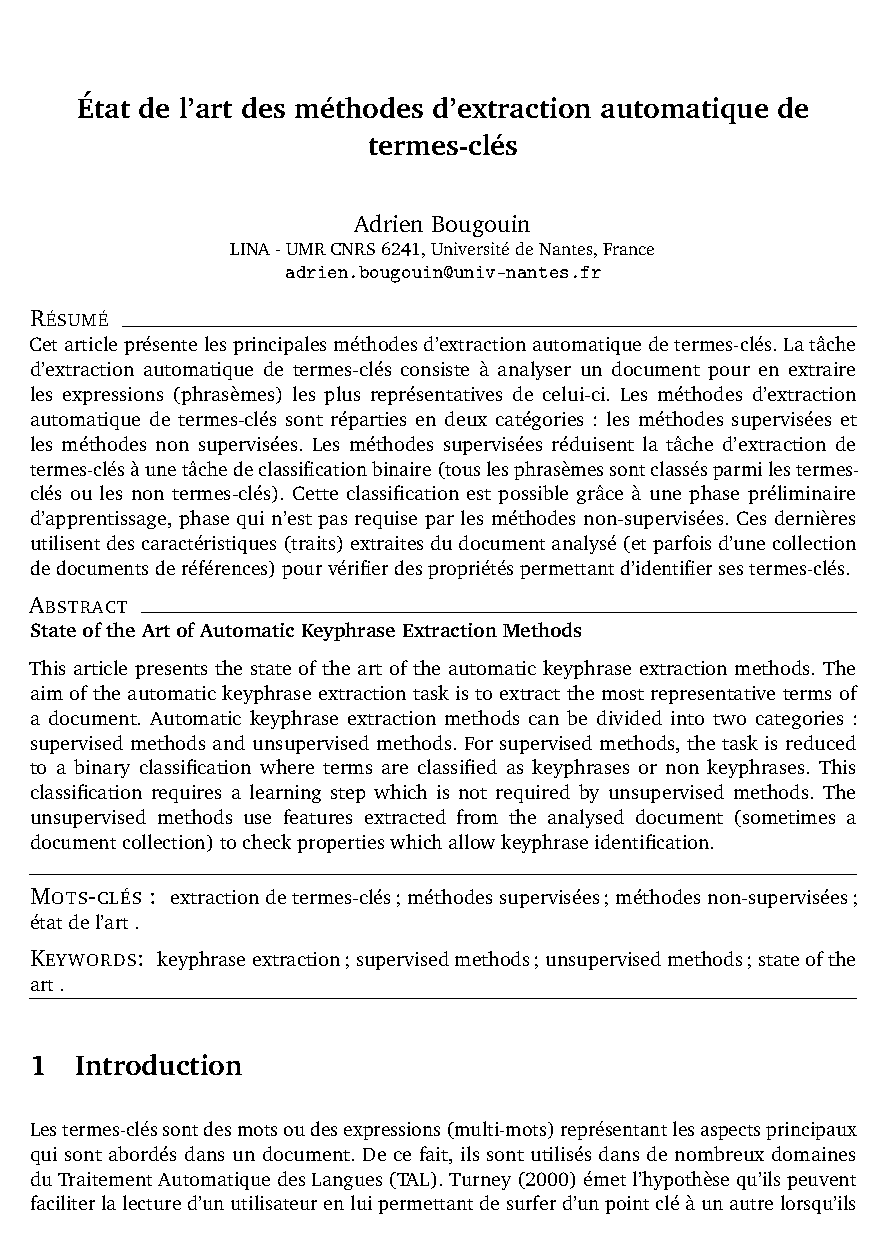
\includepdf[pages=-, templatesize={1.25\textwidth}{1.25\textheight}, frame=true, pagecommand={}]{articles/recital_2013.pdf}

      \section{\textit{TopicRank: Graph-Based Topic Ranking for Keyphrase
               Extraction}}
      \label{sec:ijcnlp2013}
        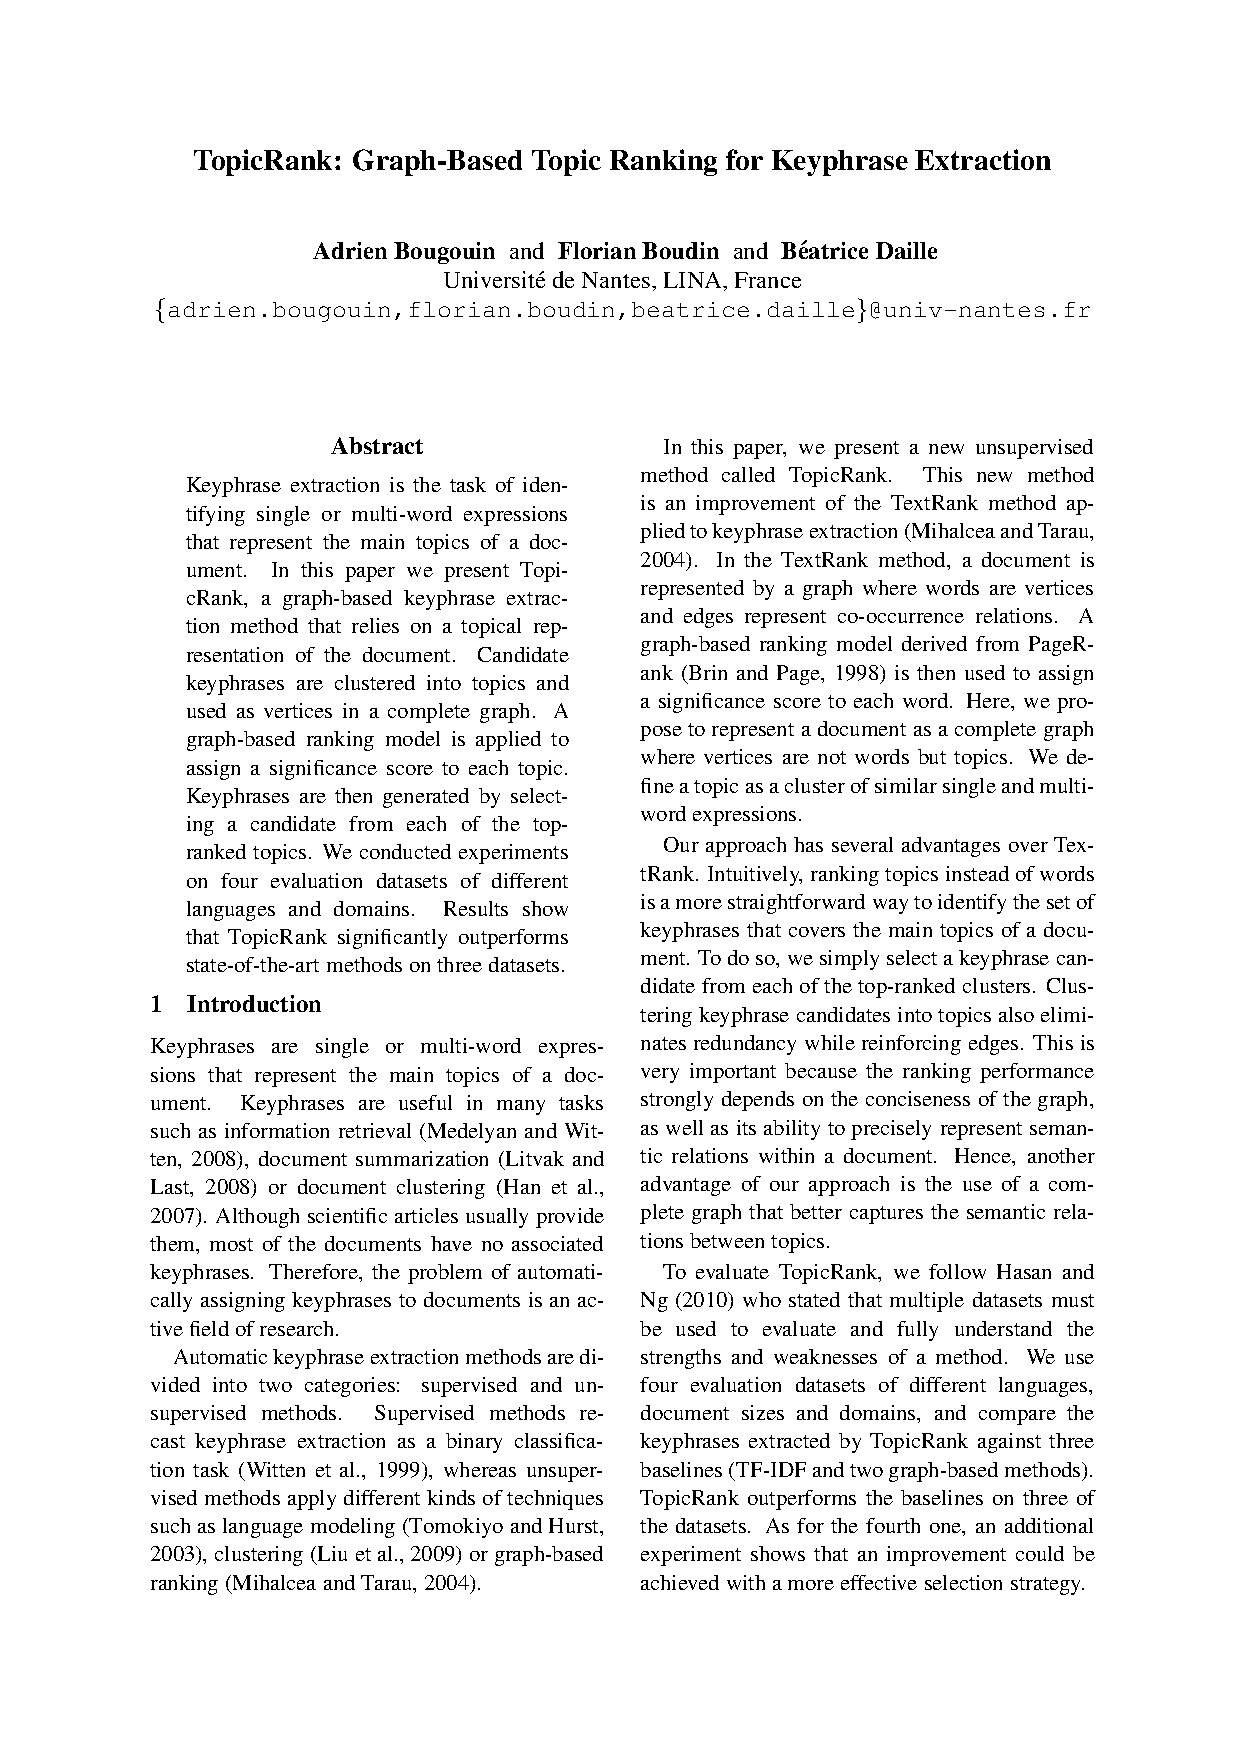
\includepdf[pages=-, templatesize={1.75\textwidth}{1.75\textheight}, frame=true, pagecommand={}]{articles/ijcnlp_2013.pdf}

    \chapter{Articles acceptés (version non-finale)}
      \section{\textit{Influence des domaines de spécialité dans l'extraction de
               termes-clés}}
      \label{sec:taln2014}
        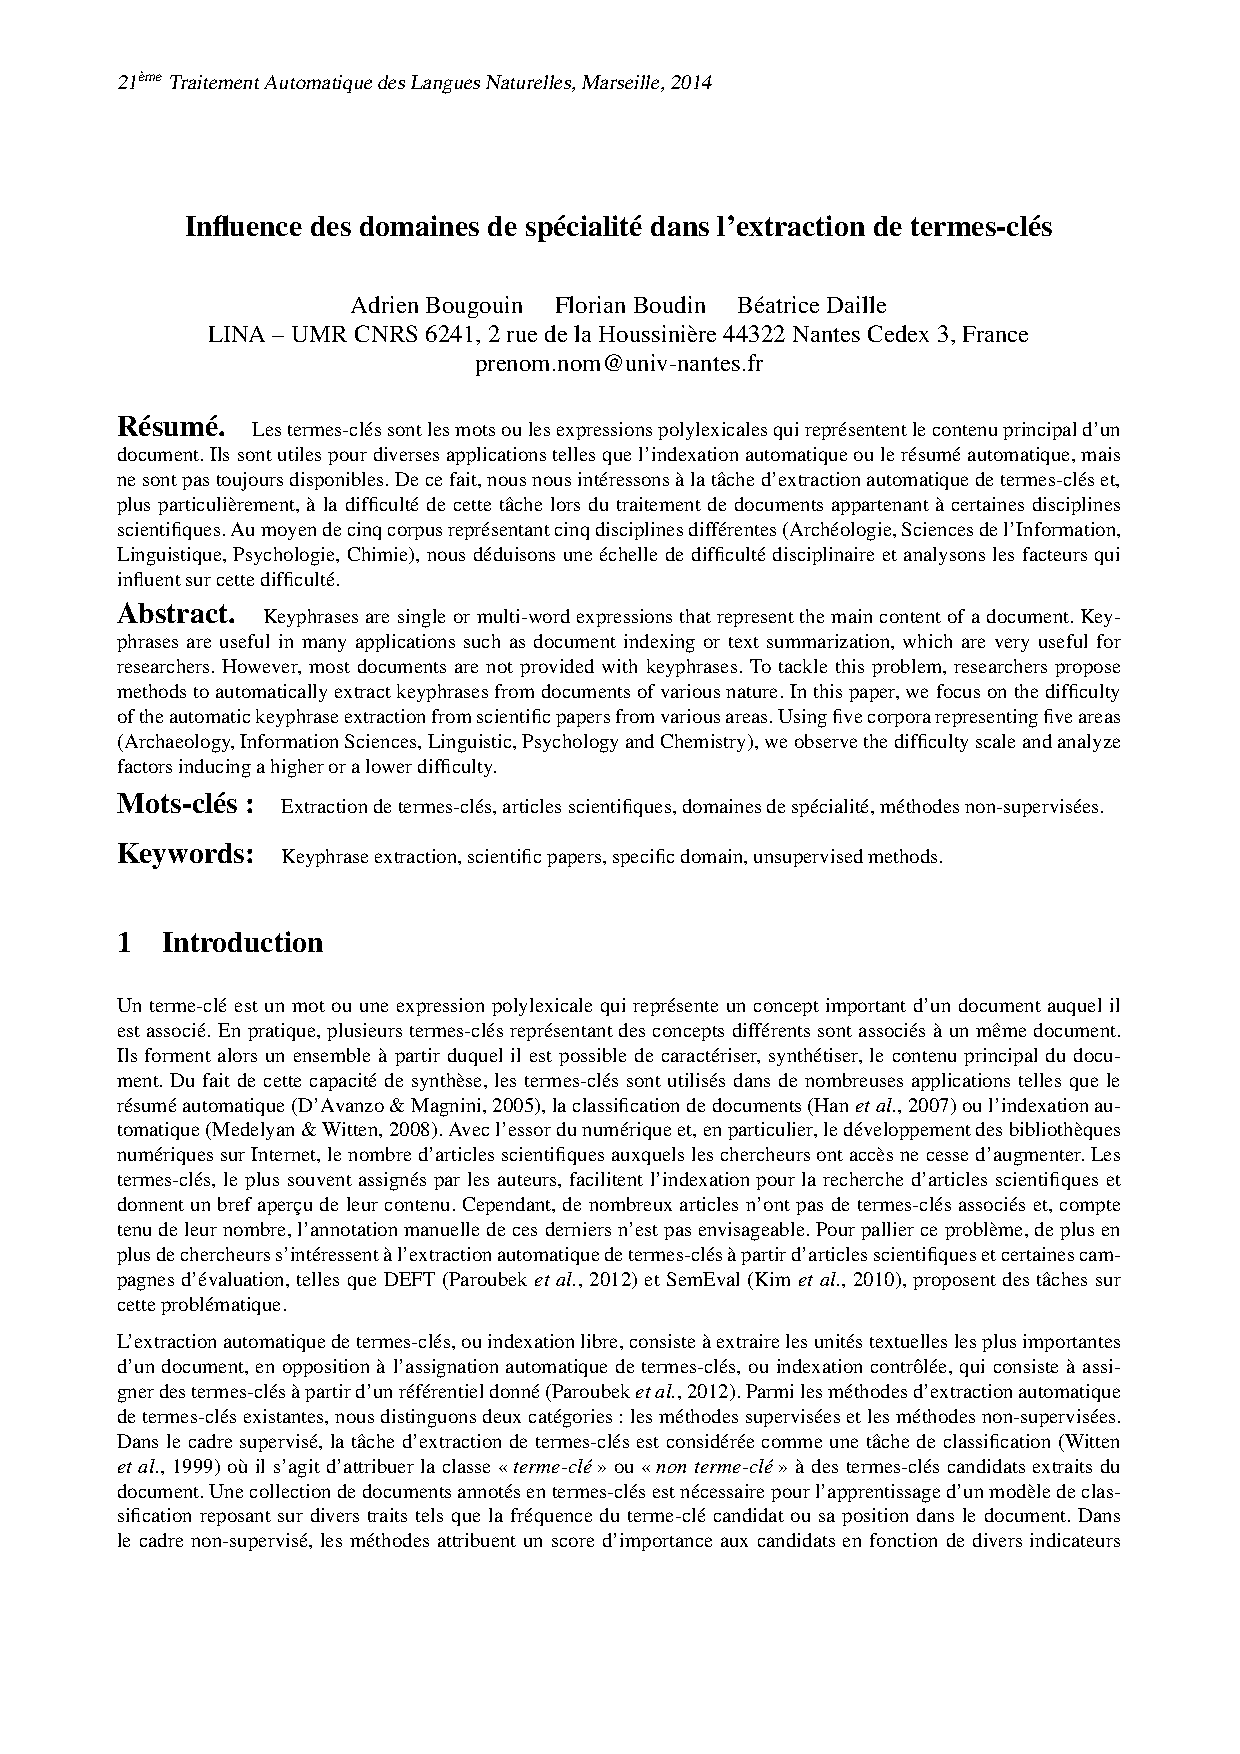
\includepdf[pages=-, templatesize={1.75\textwidth}{1.75\textheight}, frame=true, pagecommand={}]{articles/taln_2014.pdf}

    \chapter{Articles soumis (en cours de relecture)}
      \section{\textit{TopicRank : ordonnancement de sujets pour l'extraction
               automatique de termes-clés}}
      \label{sec:tal2014}
        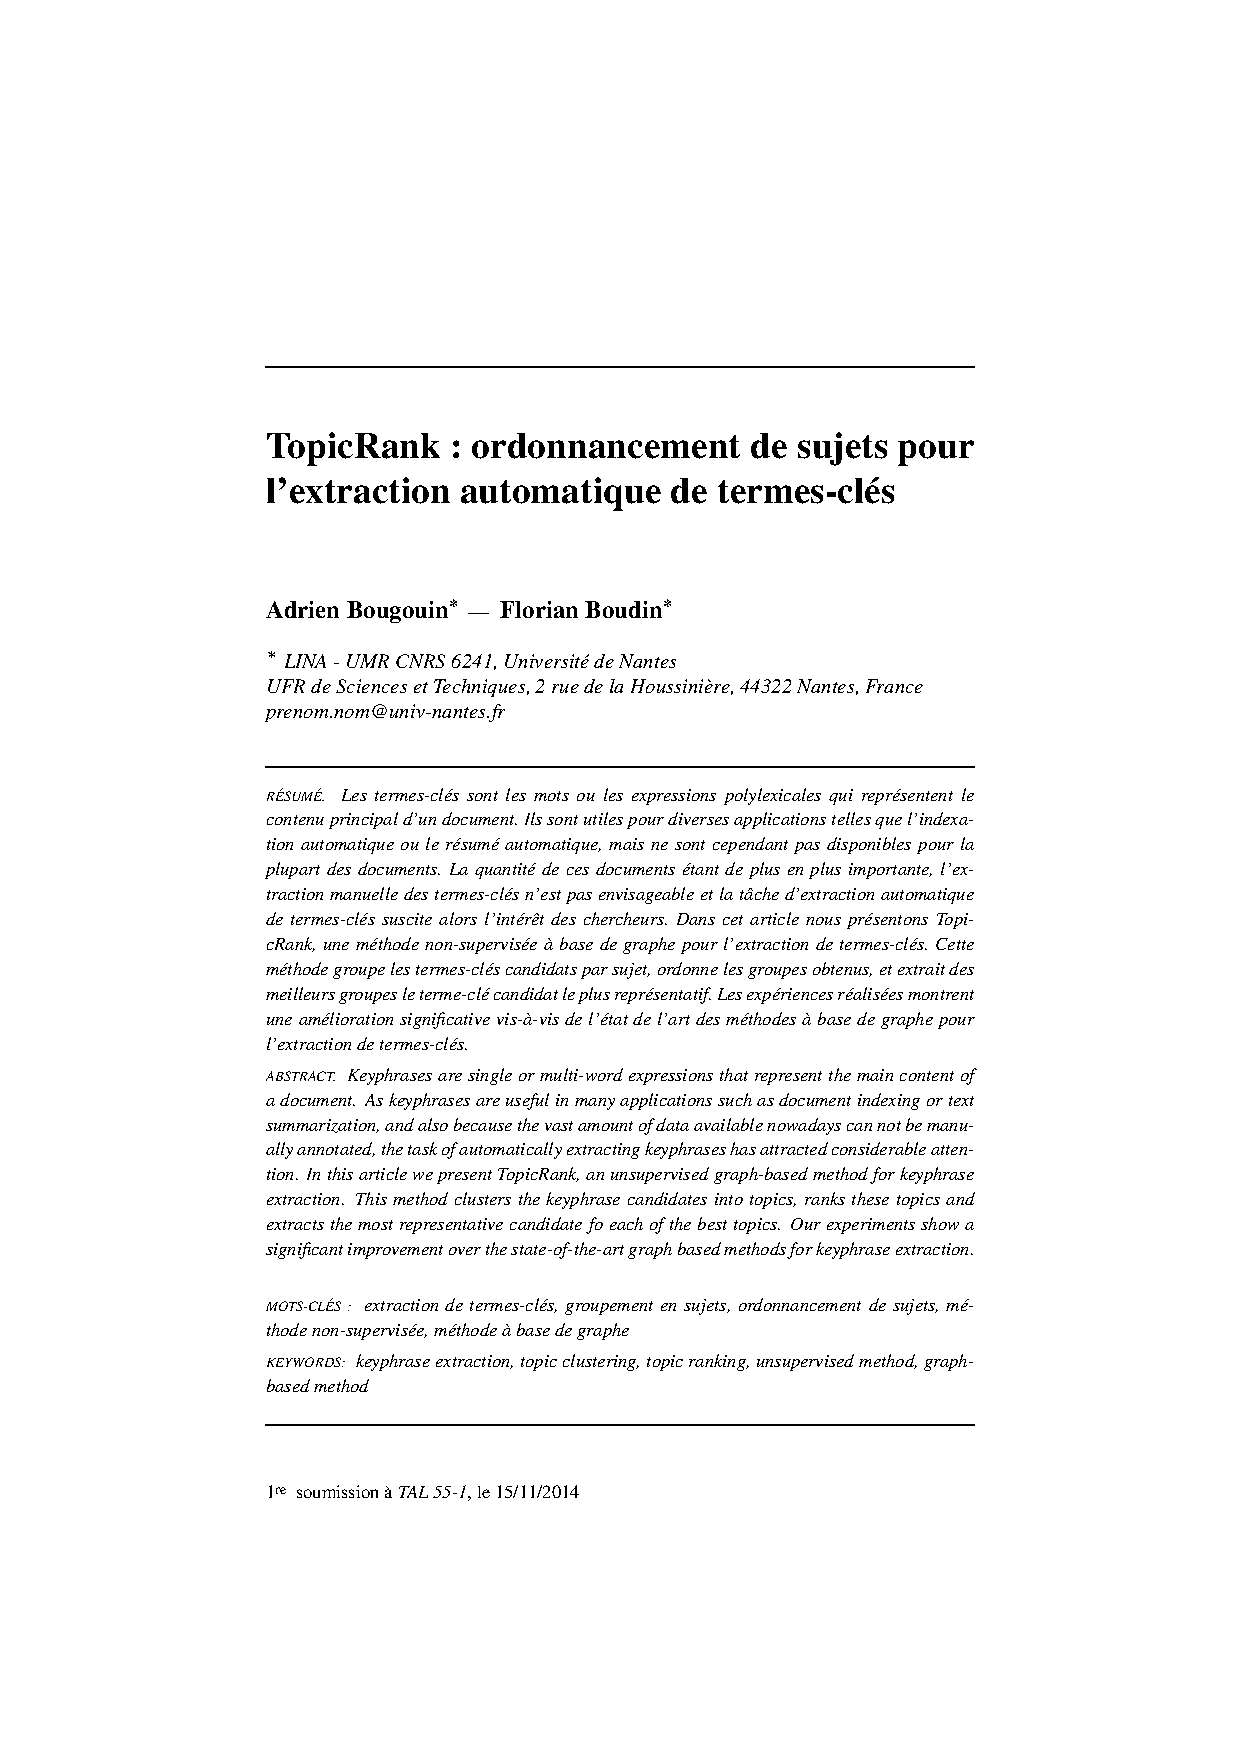
\includepdf[pages=-, templatesize={1.75\textwidth}{1.75\textheight}, frame=true, pagecommand={}]{articles/tal_2014.pdf}

      \section{\textit{Selecting Candidates for Automatic Keyphrase Extraction}}
      \label{sec:coling2014}
        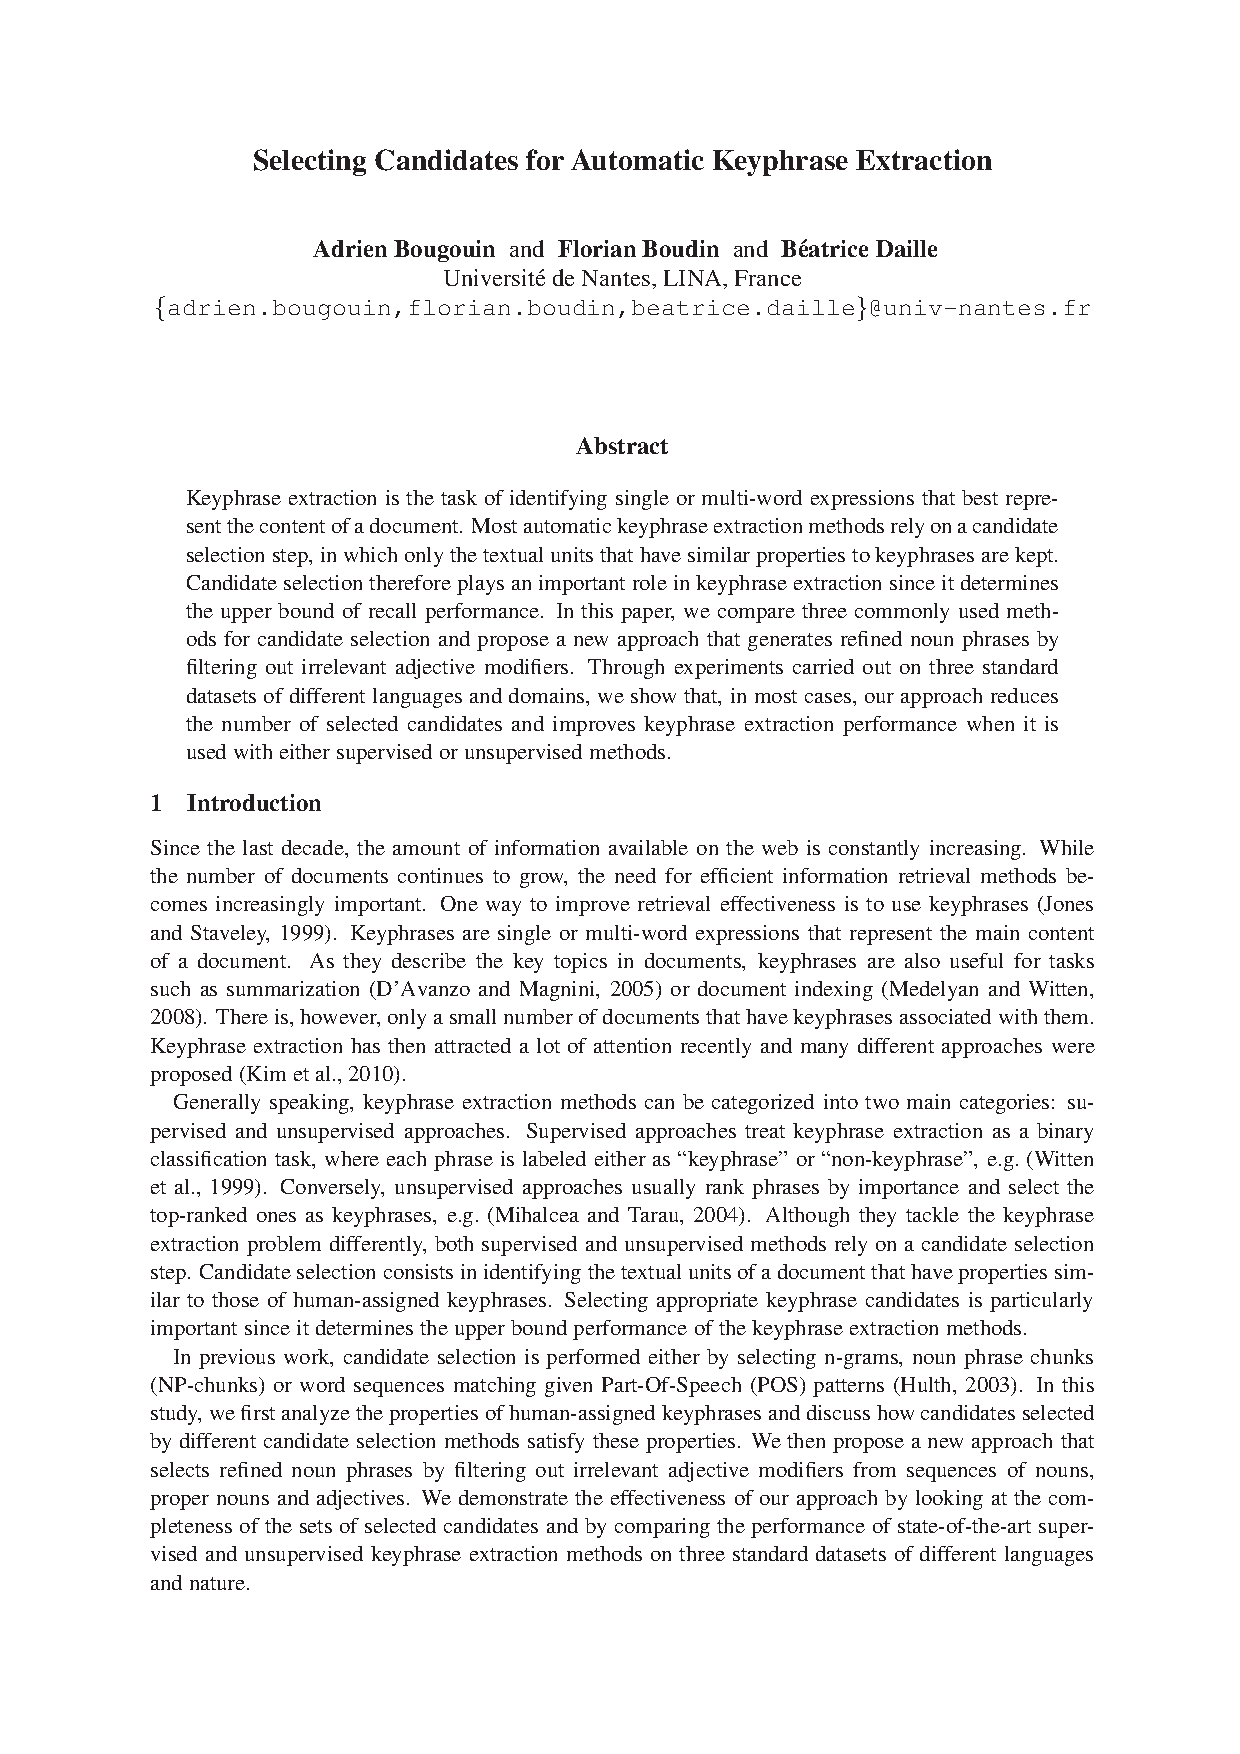
\includepdf[pages=-, templatesize={1.75\textwidth}{1.75\textheight}, frame=true, pagecommand={}]{articles/coling_2014.pdf}

\end{document}

